\subsection{Supporting Tables, Equations, and Algorithms}

\begin{longtable}[]{@{}
  >{\raggedright\arraybackslash}p{(\columnwidth - 10\tabcolsep) * \real{0.1667}}
  >{\raggedright\arraybackslash}p{(\columnwidth - 10\tabcolsep) * \real{0.1667}}
  >{\raggedright\arraybackslash}p{(\columnwidth - 10\tabcolsep) * \real{0.1667}}
  >{\raggedright\arraybackslash}p{(\columnwidth - 10\tabcolsep) * \real{0.1667}}
  >{\raggedright\arraybackslash}p{(\columnwidth - 10\tabcolsep) * \real{0.1667}}
  >{\raggedright\arraybackslash}p{(\columnwidth - 10\tabcolsep) * \real{0.1667}}@{}}
\toprule\noalign{}
\begin{minipage}[b]{\linewidth}\raggedright
Feature
\end{minipage} & \begin{minipage}[b]{\linewidth}\raggedright
AWS Security Hub
\end{minipage} & \begin{minipage}[b]{\linewidth}\raggedright
Amazon Inspector
\end{minipage} & \begin{minipage}[b]{\linewidth}\raggedright
Prowler
\end{minipage} & \begin{minipage}[b]{\linewidth}\raggedright
ScoutSuite
\end{minipage} & \begin{minipage}[b]{\linewidth}\raggedright
CloudSentinel AI (Proposed)
\end{minipage} \\
\midrule\noalign{}
\endhead
\bottomrule\noalign{}
\endlastfoot
Cloud Misconfiguration Detection & \(\checkmark\) & Partial & \(\checkmark\) & \(\checkmark\) & \(\checkmark\) \\
Vulnerability Assessment & Partial & \(\checkmark\) & Partial & Partial & \(\checkmark\) \\
Compliance Assessment & \(\checkmark\) & Partial & \(\checkmark\) & \(\checkmark\) & \(\checkmark\) \\
Knowledge Graph Modeling & \(\times\) & \(\times\) & \(\times\) & \(\times\) & \(\checkmark\) \\
Attack Graph Generation & \(\times\) & \(\times\) & \(\times\) & \(\times\) & \(\checkmark\) \\
Attack Path Analysis & \(\times\) & \(\times\) & \(\times\) & \(\times\) & \(\checkmark\) \\
Context-Aware Risk Assessment & \(\times\) & \(\times\) & \(\times\) & \(\times\) & \(\checkmark\) \\
Explainable AI Recommendations & \(\times\) & \(\times\) & \(\times\) & \(\times\) & \(\checkmark\) \\
Automated Risk Prioritization & Partial & Partial & \(\times\) & \(\times\) & \(\checkmark\) \\
Interactive Security Dashboard & \(\checkmark\) & \(\checkmark\) & Limited & Limited & \(\checkmark\) \\
Multi-Service Relationship Analysis & \(\times\) & \(\times\) & \(\times\) & \(\times\) & \(\checkmark\) \\
Continuous Monitoring & \(\checkmark\) & \(\checkmark\) & Limited & Limited & \(\checkmark\) \\
\end{longtable}

Table-2.1:Comparison of Existing Cloud Security Solutions\\
Observation:\\
The comparison indicates that existing cloud security solutions primarily focus on detecting individual vulnerabilities, compliance violations, or configuration issues. However, they lack integrated capabilities such as knowledge graph modeling, attack graph generation, context-aware risk assessment, and Explainable AI-based remediation. The proposed \textbf{CloudSentinel AI} framework addresses these gaps by combining graph-based security analysis with intelligent risk prioritization and explainable recommendations, enabling a more comprehensive cloud security assessment.

\begin{longtable}[]{@{}
  >{\raggedright\arraybackslash}p{(\columnwidth - 6\tabcolsep) * \real{0.2500}}
  >{\raggedright\arraybackslash}p{(\columnwidth - 6\tabcolsep) * \real{0.2500}}
  >{\raggedright\arraybackslash}p{(\columnwidth - 6\tabcolsep) * \real{0.2500}}
  >{\raggedright\arraybackslash}p{(\columnwidth - 6\tabcolsep) * \real{0.2500}}@{}}
\toprule\noalign{}
\begin{minipage}[b]{\linewidth}\raggedright
Threat / Misconfiguration
\end{minipage} & \begin{minipage}[b]{\linewidth}\raggedright
Description
\end{minipage} & \begin{minipage}[b]{\linewidth}\raggedright
Potential Impact
\end{minipage} & \begin{minipage}[b]{\linewidth}\raggedright
Example AWS Resource
\end{minipage} \\
\midrule\noalign{}
\endhead
\bottomrule\noalign{}
\endlastfoot
Publicly Accessible Storage & Storage resources are exposed to the internet due to improper access controls. & Data leakage, unauthorized access, compliance violations & Amazon S3 \\
Excessive IAM Permissions & IAM users or roles are granted permissions beyond the principle of least privilege. & Privilege escalation, unauthorized resource access & IAM User, IAM Role \\
Open Security Groups & Security groups allow unrestricted inbound access (e.g., SSH/RDP open to 0.0.0.0/0). & Remote exploitation, brute-force attacks & EC2 Security Group \\
Unencrypted Storage & Data is stored without encryption at rest. & Data disclosure if storage is compromised & Amazon EBS, Amazon RDS \\
Weak Authentication & Multi-Factor Authentication (MFA) is disabled or weak passwords are used. & Account compromise and unauthorized access & IAM Users \\
Misconfigured Network Routing & Incorrect route tables or network ACLs expose internal resources. & Unauthorized network access and lateral movement & VPC, Route Tables \\
Exposed Secrets and Credentials & API keys, database passwords, or tokens are improperly stored or publicly accessible. & Credential theft and service compromise & AWS Secrets Manager, Environment Variables \\
Disabled Logging and Monitoring & CloudTrail, CloudWatch, or AWS Config are disabled or improperly configured. & Reduced visibility and delayed incident detection & CloudTrail, CloudWatch \\
Vulnerable Compute Instances & EC2 instances or Lambda functions contain outdated software or known vulnerabilities. & Remote code execution and system compromise & Amazon EC2, AWS Lambda \\
Misconfigured Databases & Databases are publicly accessible or lack proper authentication and encryption. & Data theft, unauthorized modification, compliance risks & Amazon RDS, DynamoDB \\
\end{longtable}

Table-3.1:Common Cloud Security Threats and Misconfigurations\\
Observation:\\
Cloud environments are susceptible to a wide range of security threats arising from configuration errors, excessive permissions, weak authentication mechanisms, and inadequate monitoring. While each misconfiguration may appear isolated, attackers often exploit multiple weaknesses together to achieve privilege escalation, lateral movement, and unauthorized access to sensitive resources. Addressing these challenges requires a holistic security assessment framework capable of analyzing relationships among cloud resources and identifying potential attack paths.

\begin{longtable}[]{@{}
  >{\raggedright\arraybackslash}p{(\columnwidth - 6\tabcolsep) * \real{0.2500}}
  >{\raggedright\arraybackslash}p{(\columnwidth - 6\tabcolsep) * \real{0.2500}}
  >{\raggedright\arraybackslash}p{(\columnwidth - 6\tabcolsep) * \real{0.2500}}
  >{\raggedright\arraybackslash}p{(\columnwidth - 6\tabcolsep) * \real{0.2500}}@{}}
\toprule\noalign{}
\begin{minipage}[b]{\linewidth}\raggedright
Component
\end{minipage} & \begin{minipage}[b]{\linewidth}\raggedright
Primary Function
\end{minipage} & \begin{minipage}[b]{\linewidth}\raggedright
Input
\end{minipage} & \begin{minipage}[b]{\linewidth}\raggedright
Output
\end{minipage} \\
\midrule\noalign{}
\endhead
\bottomrule\noalign{}
\endlastfoot
Cloud Asset Collection Module & Discovers cloud resources and gathers configuration metadata from AWS services. & AWS APIs, Cloud Resources & Asset Inventory \\
Security Configuration Analysis Module & Detects security misconfigurations, compliance issues, and configuration weaknesses. & Asset Inventory & Security Findings \\
Knowledge Graph Construction Module & Models cloud resources and their relationships as a graph database. & Cloud Assets, Security Metadata & Knowledge Graph \\
Attack Graph Generation Module & Identifies possible attack paths based on resource relationships and security findings. & Knowledge Graph & Attack Graph \\
Context-Aware Risk Assessment Module & Calculates risk scores by considering exploitability, relationships, and business impact. & Attack Graph, Findings & Prioritized Risk Scores \\
Explainable AI Recommendation Module & Generates human-readable explanations and remediation suggestions. & Risk Scores, Security Findings & AI Recommendations \\
Dashboard \& Reporting Module & Visualizes security posture and generates assessment reports. & Analysis Results & Dashboards, Reports \\
\end{longtable}

Table-5.1:Functional Components of the CloudSentinel AI Framework\\
Observation:\\
The CloudSentinel AI framework is organized into modular components, each responsible for a specific stage of the cloud security assessment pipeline. The output of one module serves as the input to the next, enabling a seamless flow from cloud asset discovery to explainable security recommendations. This modular design improves scalability, maintainability, and future extensibility.

\begin{longtable}[]{@{}
  >{\raggedright\arraybackslash}p{(\columnwidth - 8\tabcolsep) * \real{0.2000}}
  >{\raggedright\arraybackslash}p{(\columnwidth - 8\tabcolsep) * \real{0.2000}}
  >{\raggedright\arraybackslash}p{(\columnwidth - 8\tabcolsep) * \real{0.2000}}
  >{\raggedright\arraybackslash}p{(\columnwidth - 8\tabcolsep) * \real{0.2000}}
  >{\raggedright\arraybackslash}p{(\columnwidth - 8\tabcolsep) * \real{0.2000}}@{}}
\toprule\noalign{}
\begin{minipage}[b]{\linewidth}\raggedright
Module
\end{minipage} & \begin{minipage}[b]{\linewidth}\raggedright
Responsibilities
\end{minipage} & \begin{minipage}[b]{\linewidth}\raggedright
Input
\end{minipage} & \begin{minipage}[b]{\linewidth}\raggedright
Output
\end{minipage} & \begin{minipage}[b]{\linewidth}\raggedright
Technologies / Techniques
\end{minipage} \\
\midrule\noalign{}
\endhead
\bottomrule\noalign{}
\endlastfoot
Cloud Asset Collection & Discover AWS resources and collect configuration metadata using cloud APIs. & AWS APIs & Cloud Resource Inventory & AWS SDK, Boto3 \\
Configuration Analysis & Detect security misconfigurations and evaluate compliance against security standards. & Cloud Resource Inventory & Security Findings & Rule-Based Analysis, CIS Benchmarks \\
Knowledge Graph Construction & Transform cloud resources and relationships into a graph representation. & Security Findings, Metadata & Knowledge Graph & Neo4j, Graph Modeling \\
Attack Graph Generation & Identify attack paths, privilege escalation opportunities, and lateral movement. & Knowledge Graph & Attack Graph & Graph Traversal Algorithms \\
Context-Aware Risk Assessment & Calculate risk scores based on exploitability, resource relationships, and business impact. & Attack Graph, Findings & Risk Assessment Results & Risk Scoring Model \\
Explainable AI Engine & Generate human-readable explanations and remediation recommendations. & Risk Assessment Results & AI Recommendations & Large Language Model (LLM), Explainable AI \\
Dashboard \& Reporting & Visualize security posture and generate downloadable reports. & AI Recommendations & Dashboards, PDF/CSV Reports & Web Dashboard, Reporting Engine \\
\end{longtable}

Table-6.1: CloudSentinel AI Module Specifications\\
\textbf{Observation:}

The CloudSentinel AI framework is composed of seven modular components, each responsible for a distinct stage of the cloud security assessment pipeline. This modular architecture enables efficient processing of cloud resource data while ensuring scalability, maintainability, and extensibility. The sequential interaction between modules allows the framework to transform raw cloud configurations into actionable, explainable security intelligence.

\begin{longtable}[]{@{}
  >{\raggedright\arraybackslash}p{(\columnwidth - 4\tabcolsep) * \real{0.3333}}
  >{\raggedright\arraybackslash}p{(\columnwidth - 4\tabcolsep) * \real{0.3333}}
  >{\raggedright\arraybackslash}p{(\columnwidth - 4\tabcolsep) * \real{0.3333}}@{}}
\toprule\noalign{}
\begin{minipage}[b]{\linewidth}\raggedright
Layer
\end{minipage} & \begin{minipage}[b]{\linewidth}\raggedright
Technology
\end{minipage} & \begin{minipage}[b]{\linewidth}\raggedright
Purpose
\end{minipage} \\
\midrule\noalign{}
\endhead
\bottomrule\noalign{}
\endlastfoot
Cloud Platform & Amazon Web Services (AWS) & Provides cloud infrastructure and services for security assessment. \\
Programming Language & Python & Core implementation of CloudSentinel AI framework. \\
Backend Framework & FastAPI & Develops RESTful APIs and manages communication between system modules. \\
Cloud SDK & Boto3 (AWS SDK for Python) & Collects cloud resource information and configuration metadata. \\
Graph Database & Neo4j & Stores cloud resources and their relationships as a knowledge graph. \\
Relational Database & PostgreSQL & Stores user information, scan history, findings, and reports. \\
Graph Analytics & Neo4j Graph Data Science (GDS) & Performs graph traversal and attack path analysis. \\
AI Engine & Large Language Model (LLM) & Generates explainable risk assessments and remediation recommendations. \\
Visualization & React.js & Provides an interactive web-based security dashboard. \\
Containerization & Docker & Packages and deploys application components consistently. \\
Version Control & Git \& GitHub & Manages source code and collaborative development. \\
Development Environment & Visual Studio Code & Integrated development environment used for implementation. \\
\end{longtable}

Table-8.1:Software and Technology Stack Used in CloudSentinel AI

\textbf{Observation:}

The CloudSentinel AI framework integrates modern cloud-native and graph-based technologies to provide a scalable and intelligent cloud security assessment platform. AWS serves as the target cloud environment, while Python and FastAPI implement the core backend services. Neo4j enables relationship modeling and attack path analysis, PostgreSQL stores structured application data, and a Large Language Model (LLM) provides explainable AI-driven remediation recommendations. Docker ensures consistent deployment across development and production environments.

\begin{longtable}[]{@{}
  >{\raggedright\arraybackslash}p{(\columnwidth - 6\tabcolsep) * \real{0.2500}}
  >{\raggedright\arraybackslash}p{(\columnwidth - 6\tabcolsep) * \real{0.2500}}
  >{\raggedright\arraybackslash}p{(\columnwidth - 6\tabcolsep) * \real{0.2500}}
  >{\raggedright\arraybackslash}p{(\columnwidth - 6\tabcolsep) * \real{0.2500}}@{}}
\toprule\noalign{}
\begin{minipage}[b]{\linewidth}\raggedright
Component
\end{minipage} & \begin{minipage}[b]{\linewidth}\raggedright
Technology / Tool
\end{minipage} & \begin{minipage}[b]{\linewidth}\raggedright
Role in the Framework
\end{minipage} & \begin{minipage}[b]{\linewidth}\raggedright
Reason for Selection
\end{minipage} \\
\midrule\noalign{}
\endhead
\bottomrule\noalign{}
\endlastfoot
Cloud Resource Discovery & AWS SDK (Boto3) & Collects AWS resource metadata and configurations & Official AWS SDK with comprehensive API support \\
Knowledge Graph & Neo4j & Represents cloud assets and their relationships & Efficient storage and querying of highly connected data \\
Graph Analytics & Neo4j Graph Data Science (GDS) & Performs graph traversal and attack path analysis & Optimized graph algorithms for security analysis \\
Security Analysis & Rule-Based Engine & Detects cloud misconfigurations and policy violations & Supports deterministic and explainable security checks \\
AI Recommendation Engine & Large Language Model (LLM) & Generates explainable security recommendations & Produces human-readable explanations and remediation guidance \\
Risk Assessment & Context-Aware Risk Scoring Model & Calculates security risk based on multiple factors & Prioritizes findings using contextual information instead of isolated alerts \\
Backend Services & FastAPI & Hosts APIs and coordinates system modules & High-performance asynchronous web framework \\
Data Storage & PostgreSQL & Stores scan history, reports, and application data & Reliable relational database with strong transactional support \\
User Interface & React.js & Displays dashboards and security reports & Enables responsive and interactive web applications \\
Deployment & Docker & Packages and deploys framework components & Ensures portability and reproducible deployments \\
\end{longtable}

Table-8.2:AI Models, Graph Technologies, and Supporting Tools Used in CloudSentinel AI

\textbf{Observation:}

CloudSentinel AI combines graph technologies, artificial intelligence, and cloud-native tools to build an integrated cloud security assessment framework. Neo4j enables relationship-aware analysis of cloud resources, while Graph Data Science algorithms support attack path identification. The explainable AI module provides contextual remediation recommendations, and FastAPI, PostgreSQL, React.js, and Docker collectively ensure a scalable, maintainable, and portable implementation.

\begin{longtable}[]{@{}
  >{\raggedright\arraybackslash}p{(\columnwidth - 6\tabcolsep) * \real{0.2500}}
  >{\raggedright\arraybackslash}p{(\columnwidth - 6\tabcolsep) * \real{0.2500}}
  >{\raggedright\arraybackslash}p{(\columnwidth - 6\tabcolsep) * \real{0.2500}}
  >{\raggedright\arraybackslash}p{(\columnwidth - 6\tabcolsep) * \real{0.2500}}@{}}
\toprule\noalign{}
\begin{minipage}[b]{\linewidth}\raggedright
Entity
\end{minipage} & \begin{minipage}[b]{\linewidth}\raggedright
Description
\end{minipage} & \begin{minipage}[b]{\linewidth}\raggedright
Primary Attributes
\end{minipage} & \begin{minipage}[b]{\linewidth}\raggedright
Relationships
\end{minipage} \\
\midrule\noalign{}
\endhead
\bottomrule\noalign{}
\endlastfoot
User & Stores information about authenticated users of the framework. & User ID, Name, Email, Password, Role & Creates and manages cloud scan projects \\
Cloud Project & Represents a cloud environment or AWS account being assessed. & Project ID, Project Name, AWS Account ID, Region & Contains multiple security scans \\
Security Scan & Records each execution of a cloud security assessment. & Scan ID, Scan Date, Scan Status, Duration & Generates findings and reports \\
Cloud Resource & Stores metadata of discovered cloud resources. & Resource ID, Resource Type, Resource Name, Region & Associated with security findings and graph nodes \\
Security Finding & Stores identified vulnerabilities and misconfigurations. & Finding ID, Severity, Category, Description & Linked to cloud resources and risk assessments \\
Risk Assessment & Stores calculated contextual risk scores for findings. & Risk ID, Risk Score, Priority, Status & References security findings and AI recommendations \\
AI Recommendation & Stores explainable remediation suggestions generated by the AI module. & Recommendation ID, Recommendation Text, Confidence Score & Associated with risk assessments \\
Assessment Report & Stores generated security reports and summaries. & Report ID, Report Name, Generated Date, Report Format & Created from completed security scans \\
\end{longtable}

Table-9.1:Database Entity Summary of CloudSentinel AI\\
\textbf{Observation:}

The CloudSentinel AI database is designed using a relational model to efficiently manage user information, cloud projects, scan history, discovered resources, security findings, risk assessments, AI-generated recommendations, and assessment reports. This structured design ensures data consistency while enabling seamless integration with the knowledge graph stored in Neo4j. The separation of operational data from graph data improves scalability, simplifies maintenance, and supports efficient querying across different system components.

\begin{longtable}[]{@{}
  >{\raggedright\arraybackslash}p{(\columnwidth - 6\tabcolsep) * \real{0.2500}}
  >{\raggedright\arraybackslash}p{(\columnwidth - 6\tabcolsep) * \real{0.2500}}
  >{\raggedright\arraybackslash}p{(\columnwidth - 6\tabcolsep) * \real{0.2500}}
  >{\raggedright\arraybackslash}p{(\columnwidth - 6\tabcolsep) * \real{0.2500}}@{}}
\toprule\noalign{}
\begin{minipage}[b]{\linewidth}\raggedright
Node Type
\end{minipage} & \begin{minipage}[b]{\linewidth}\raggedright
Description
\end{minipage} & \begin{minipage}[b]{\linewidth}\raggedright
Key Properties
\end{minipage} & \begin{minipage}[b]{\linewidth}\raggedright
Primary Relationships
\end{minipage} \\
\midrule\noalign{}
\endhead
\bottomrule\noalign{}
\endlastfoot
AWS Account & Represents the AWS account being assessed. & Account ID, Account Name & CONTAINS \\
VPC & Represents a Virtual Private Cloud. & VPC ID, CIDR Block, Region & CONTAINS, CONNECTED\_TO \\
Subnet & Represents a subnet within a VPC. & Subnet ID, CIDR Block, Availability Zone & BELONGS\_TO, HOSTS \\
EC2 Instance & Represents a virtual machine instance. & Instance ID, Name, State, Public IP & HOSTED\_IN, USES\_ROLE, PROTECTED\_BY \\
IAM User & Represents an AWS Identity and Access Management user. & User ID, User Name & ASSUMES\_ROLE, HAS\_PERMISSION \\
IAM Role & Represents an IAM role assigned to services or users. & Role ID, Role Name & GRANTS\_PERMISSION, ASSIGNED\_TO \\
Security Group & Represents firewall rules controlling network traffic. & Group ID, Group Name & PROTECTS, ALLOWS\_ACCESS\_TO \\
S3 Bucket & Represents cloud object storage. & Bucket Name, Encryption Status & STORES\_DATA, ACCESSIBLE\_BY \\
RDS Instance & Represents a managed relational database. & Database ID, Engine, Endpoint & CONNECTED\_TO \\
Lambda Function & Represents a serverless compute function. & Function Name, Runtime & INVOKES, ACCESSES \\
CloudTrail & Represents audit logging services. & Trail Name, Logging Status & MONITORS \\
Security Finding & Represents detected vulnerabilities or misconfigurations. & Finding ID, Severity, Category & AFFECTS \\
Risk Assessment & Represents calculated contextual risk. & Risk Score, Priority & GENERATED\_FROM \\
AI Recommendation & Represents AI-generated remediation guidance. & Recommendation ID, Confidence Score & RECOMMENDS \\
\end{longtable}

Table-9.2:Neo4j Node and Relationship Types in the CloudSentinel AI Knowledge Graph\\
\textbf{Observation:}

The CloudSentinel AI knowledge graph models AWS resources, identities, security controls, findings, and risk assessments as interconnected nodes and relationships. Unlike traditional relational representations, the property graph model captures dependencies and interactions among cloud assets, enabling efficient graph traversal, attack path generation, and context-aware risk analysis. This representation forms the foundation for identifying multi-stage attack paths and generating explainable security insights.

\begin{center}\rule{0.5\linewidth}{0.5pt}\end{center}

\begin{longtable}[]{@{}
  >{\raggedright\arraybackslash}p{(\columnwidth - 4\tabcolsep) * \real{0.3333}}
  >{\raggedright\arraybackslash}p{(\columnwidth - 4\tabcolsep) * \real{0.3333}}
  >{\raggedright\arraybackslash}p{(\columnwidth - 4\tabcolsep) * \real{0.3333}}@{}}
\toprule\noalign{}
\begin{minipage}[b]{\linewidth}\raggedright
Component
\end{minipage} & \begin{minipage}[b]{\linewidth}\raggedright
Configuration
\end{minipage} & \begin{minipage}[b]{\linewidth}\raggedright
Purpose
\end{minipage} \\
\midrule\noalign{}
\endhead
\bottomrule\noalign{}
\endlastfoot
Cloud Provider & Amazon Web Services (AWS) & Primary cloud platform used for experimental evaluation \\
Region & ap-south-1 (Mumbai) \emph{(or the region you used)} & Deployment location for all AWS resources \\
Virtual Network & Amazon VPC & Isolates and manages the experimental cloud environment \\
Compute Service & Amazon EC2 (t3.medium) \emph{(or your instance type)} & Hosts vulnerable workloads and application services \\
Storage Service & Amazon S3 & Stores application data and evaluates storage misconfigurations \\
Identity Management & AWS IAM & Configures users, roles, and permission policies \\
Database Service & Amazon RDS (PostgreSQL) & Stores relational application and experimental data \\
Logging \& Monitoring & AWS CloudTrail, Amazon CloudWatch & Captures audit logs and monitors cloud activities \\
Knowledge Graph Database & Neo4j Community Edition & Stores cloud assets and resource relationships \\
Backend Server & FastAPI (Python 3.x) & Executes security analysis and exposes REST APIs \\
Relational Database & PostgreSQL & Stores users, scan history, findings, and reports \\
Client Interface & React.js & Provides the web-based CloudSentinel AI dashboard \\
Containerization & Docker & Packages and deploys application components consistently \\
Operating System & Ubuntu 24.04 LTS & Operating system used for application deployment \\
\end{longtable}

Table 10.1 AWS Experimental Environment Configuration

\textbf{Observation:}

The experimental environment was deployed on Amazon Web Services to emulate a realistic enterprise cloud infrastructure. Core AWS services---including EC2, S3, IAM, VPC, RDS, CloudTrail, and CloudWatch---were configured to create representative cloud scenarios. CloudSentinel AI was implemented using Python, FastAPI, Neo4j, PostgreSQL, and React.js, with Docker used for containerized deployment. This environment enabled the evaluation of cloud asset discovery, misconfiguration detection, attack path generation, context-aware risk assessment, and explainable AI recommendations under realistic conditions.

\begin{longtable}[]{@{}
  >{\raggedright\arraybackslash}p{(\columnwidth - 8\tabcolsep) * \real{0.2000}}
  >{\raggedright\arraybackslash}p{(\columnwidth - 8\tabcolsep) * \real{0.2000}}
  >{\raggedright\arraybackslash}p{(\columnwidth - 8\tabcolsep) * \real{0.2000}}
  >{\raggedright\arraybackslash}p{(\columnwidth - 8\tabcolsep) * \real{0.2000}}
  >{\raggedright\arraybackslash}p{(\columnwidth - 8\tabcolsep) * \real{0.2000}}@{}}
\toprule\noalign{}
\begin{minipage}[b]{\linewidth}\raggedright
Experiment ID
\end{minipage} & \begin{minipage}[b]{\linewidth}\raggedright
Misconfiguration
\end{minipage} & \begin{minipage}[b]{\linewidth}\raggedright
Affected AWS Service
\end{minipage} & \begin{minipage}[b]{\linewidth}\raggedright
Security Risk
\end{minipage} & \begin{minipage}[b]{\linewidth}\raggedright
Expected CloudSentinel AI Detection
\end{minipage} \\
\midrule\noalign{}
\endhead
\bottomrule\noalign{}
\endlastfoot
E1 & Publicly Accessible S3 Bucket & Amazon S3 & Data exposure and unauthorized access & Detect public bucket, identify affected assets, and recommend restricting public access \\
E2 & Security Group Allowing SSH (0.0.0.0/0) & Amazon EC2 & Unauthorized remote access and brute-force attacks & Detect unrestricted inbound SSH access and prioritize remediation \\
E3 & Overly Permissive IAM Role (AdministratorAccess) & AWS IAM & Privilege escalation & Identify excessive permissions and highlight potential attack paths \\
E4 & Publicly Accessible RDS Instance & Amazon RDS & Database exposure and data leakage & Detect public database endpoint and recommend network restrictions \\
E5 & Disabled CloudTrail Logging & AWS CloudTrail & Reduced audit visibility & Identify disabled logging and recommend enabling audit trails \\
E6 & Unencrypted EBS Volume & Amazon EBS & Data disclosure if storage is compromised & Detect missing encryption and recommend enabling encryption at rest \\
E7 & IAM User Without Multi-Factor Authentication (MFA) & AWS IAM & Account compromise & Identify missing MFA and classify as an authentication weakness \\
E8 & Exposed Secrets in Secrets Manager Access Policy & AWS Secrets Manager & Credential theft & Detect excessive access permissions and recommend least-privilege policies \\
E9 & Overly Permissive Network ACL & Amazon VPC & Increased network attack surface & Detect insecure network rules and recommend restricting unnecessary traffic \\
E10 & EC2 Instance Running Outdated Software & Amazon EC2 & Exploitation of known vulnerabilities & Identify vulnerable compute instances and prioritize patch management \\
\end{longtable}

Table 10.2 Injected Cloud Security Misconfigurations for Experimental Evaluation\\
\textbf{Observation:}

To evaluate the effectiveness of CloudSentinel AI, representative cloud security misconfigurations were intentionally introduced into the AWS experimental environment. These scenarios cover identity management, network security, storage security, database exposure, monitoring, encryption, and compute security. Each experiment assesses the framework's ability to detect misconfigurations, model affected resources within the knowledge graph, generate potential attack paths, calculate contextual risk scores, and provide explainable remediation recommendations.

\begin{longtable}[]{@{}
  >{\raggedright\arraybackslash}p{(\columnwidth - 4\tabcolsep) * \real{0.3333}}
  >{\raggedright\arraybackslash}p{(\columnwidth - 4\tabcolsep) * \real{0.3333}}
  >{\raggedright\arraybackslash}p{(\columnwidth - 4\tabcolsep) * \real{0.3333}}@{}}
\toprule\noalign{}
\begin{minipage}[b]{\linewidth}\raggedright
Evaluation Metric
\end{minipage} & \begin{minipage}[b]{\linewidth}\raggedright
Definition
\end{minipage} & \begin{minipage}[b]{\linewidth}\raggedright
Purpose in CloudSentinel AI Evaluation
\end{minipage} \\
\midrule\noalign{}
\endhead
\bottomrule\noalign{}
\endlastfoot
Detection Rate (\%) & Percentage of injected cloud misconfigurations correctly identified by the framework. & Measures the effectiveness of security misconfiguration detection. \\
Precision & Ratio of correctly identified security findings to the total findings reported. & Evaluates the accuracy of generated security alerts by minimizing false positives. \\
Recall & Ratio of correctly detected security findings to the total actual security issues present. & Measures the framework's ability to identify all existing security issues. \\
F1-Score & Harmonic mean of Precision and Recall. & Provides a balanced assessment of detection performance. \\
False Positive Rate & Percentage of reported findings that are not actual security issues. & Evaluates the reliability of security alerts. \\
Risk Assessment Accuracy & Degree to which calculated risk scores align with expected security severity. & Measures the effectiveness of context-aware risk prioritization. \\
Attack Path Generation Time & Time required to construct attack graphs from the knowledge graph. & Evaluates the computational efficiency of graph analysis. \\
Knowledge Graph Construction Time & Time required to build the cloud knowledge graph from collected resources. & Measures graph generation performance and scalability. \\
AI Recommendation Response Time & Time required to generate explainable remediation recommendations. & Evaluates responsiveness of the AI module. \\
Overall Framework Execution Time & Total time required to complete a full cloud security assessment. & Measures end-to-end system performance and operational efficiency. \\
\end{longtable}

Table 10.3 Performance Evaluation Metrics Used for CloudSentinel AI\\
\textbf{Observation:}

The performance of CloudSentinel AI was evaluated using metrics that assess detection accuracy, computational efficiency, contextual risk assessment, and AI-generated recommendations. Detection Rate, Precision, Recall, and F1-Score quantify the framework's ability to accurately identify cloud security issues. Execution-time metrics evaluate the efficiency of knowledge graph construction, attack graph generation, and AI-based recommendation generation. Together, these metrics provide a comprehensive evaluation of the framework's effectiveness and scalability.

\begin{longtable}[]{@{}
  >{\raggedright\arraybackslash}p{(\columnwidth - 6\tabcolsep) * \real{0.2500}}
  >{\raggedright\arraybackslash}p{(\columnwidth - 6\tabcolsep) * \real{0.2500}}
  >{\raggedright\arraybackslash}p{(\columnwidth - 6\tabcolsep) * \real{0.2500}}
  >{\raggedright\arraybackslash}p{(\columnwidth - 6\tabcolsep) * \real{0.2500}}@{}}
\toprule\noalign{}
\begin{minipage}[b]{\linewidth}\raggedright
Scenario ID
\end{minipage} & \begin{minipage}[b]{\linewidth}\raggedright
Experimental Scenario
\end{minipage} & \begin{minipage}[b]{\linewidth}\raggedright
Validation Objective
\end{minipage} & \begin{minipage}[b]{\linewidth}\raggedright
Expected Framework Outcome
\end{minipage} \\
\midrule\noalign{}
\endhead
\bottomrule\noalign{}
\endlastfoot
S1 & Public S3 Bucket & Validate storage misconfiguration detection & Detect public access, assign risk score, and recommend restricting bucket permissions \\
S2 & Open SSH Port (0.0.0.0/0) & Validate network security analysis & Identify exposed security group, generate attack path, and prioritize remediation \\
S3 & Overly Permissive IAM Role & Validate identity and access analysis & Detect excessive privileges and identify privilege escalation opportunities \\
S4 & Publicly Accessible RDS Instance & Validate database exposure detection & Detect public database access and recommend network isolation \\
S5 & Disabled CloudTrail Logging & Validate monitoring and auditing assessment & Detect missing audit logging and recommend enabling CloudTrail \\
S6 & Unencrypted EBS Volume & Validate encryption compliance analysis & Detect missing encryption and classify the finding based on data sensitivity \\
S7 & IAM User Without MFA & Validate authentication security assessment & Identify authentication weakness and recommend enabling MFA \\
S8 & Excessive Secrets Manager Access & Validate secrets management security & Detect over-permissive access policies and recommend least-privilege permissions \\
S9 & Multi-Service Attack Chain (IAM \(\rightarrow\) EC2 \(\rightarrow\) RDS) & Validate knowledge graph and attack graph generation & Construct multi-stage attack path and calculate contextual risk score \\
S10 & Complete Enterprise Cloud Environment & Validate end-to-end framework performance & Discover assets, detect findings, generate attack graph, calculate risks, and produce AI recommendations \\
\end{longtable}

Table 10.4 Experimental Test Scenarios and Validation Objectives\\
\textbf{Observation:}

The experimental scenarios were designed to evaluate each functional capability of CloudSentinel AI individually and collectively. Initial scenarios validate the detection of common cloud misconfigurations, while later scenarios assess relationship-aware analysis through knowledge graph modeling and attack path generation. The final scenario evaluates the complete framework by performing an end-to-end cloud security assessment, demonstrating the integration of asset discovery, graph analytics, contextual risk assessment, and explainable AI recommendations.

\begin{longtable}[]{@{}
  >{\raggedright\arraybackslash}p{(\columnwidth - 10\tabcolsep) * \real{0.1667}}
  >{\raggedright\arraybackslash}p{(\columnwidth - 10\tabcolsep) * \real{0.1667}}
  >{\raggedright\arraybackslash}p{(\columnwidth - 10\tabcolsep) * \real{0.1667}}
  >{\raggedright\arraybackslash}p{(\columnwidth - 10\tabcolsep) * \real{0.1667}}
  >{\raggedright\arraybackslash}p{(\columnwidth - 10\tabcolsep) * \real{0.1667}}
  >{\raggedright\arraybackslash}p{(\columnwidth - 10\tabcolsep) * \real{0.1667}}@{}}
\toprule\noalign{}
\begin{minipage}[b]{\linewidth}\raggedright
Evaluation Criterion
\end{minipage} & \begin{minipage}[b]{\linewidth}\raggedright
AWS Security Hub
\end{minipage} & \begin{minipage}[b]{\linewidth}\raggedright
Amazon Inspector
\end{minipage} & \begin{minipage}[b]{\linewidth}\raggedright
Prowler
\end{minipage} & \begin{minipage}[b]{\linewidth}\raggedright
ScoutSuite
\end{minipage} & \begin{minipage}[b]{\linewidth}\raggedright
CloudSentinel AI (Proposed)
\end{minipage} \\
\midrule\noalign{}
\endhead
\bottomrule\noalign{}
\endlastfoot
Cloud Misconfiguration Detection & \(\checkmark\) & Partial & \(\checkmark\) & \(\checkmark\) & \(\checkmark\) \\
Vulnerability Assessment & Partial & \(\checkmark\) & Partial & Partial & \(\checkmark\) \\
Compliance Assessment & \(\checkmark\) & Partial & \(\checkmark\) & \(\checkmark\) & \(\checkmark\) \\
Knowledge Graph Modeling & \(\times\) & \(\times\) & \(\times\) & \(\times\) & \(\checkmark\) \\
Attack Graph Generation & \(\times\) & \(\times\) & \(\times\) & \(\times\) & \(\checkmark\) \\
Multi-Service Relationship Analysis & \(\times\) & \(\times\) & Limited & Limited & \(\checkmark\) \\
Context-Aware Risk Assessment & Limited & Limited & \(\times\) & \(\times\) & \(\checkmark\) \\
Explainable AI Recommendations & \(\times\) & \(\times\) & \(\times\) & \(\times\) & \(\checkmark\) \\
Automated Risk Prioritization & \(\checkmark\) & Partial & Partial & Partial & \(\checkmark\) \\
Interactive Security Dashboard & \(\checkmark\) & \(\checkmark\) & Limited & Limited & \(\checkmark\) \\
Extensible Architecture & Limited & Limited & \(\checkmark\) & \(\checkmark\) & \(\checkmark\) \\
End-to-End Security Assessment Workflow & Partial & Partial & Partial & Partial & \(\checkmark\) \\
\end{longtable}

Table 11.1 Comparative Performance Analysis of CloudSentinel AI and Existing Cloud Security Solutions\\
\textbf{Observation:}

The comparison highlights that existing cloud security solutions primarily focus on vulnerability assessment, compliance monitoring, or security configuration analysis. While these tools provide valuable capabilities, they generally do not integrate relationship-aware knowledge graph modeling, attack graph generation, contextual risk assessment, and explainable AI within a single framework. CloudSentinel AI combines these capabilities into a unified architecture, enabling more comprehensive cloud security analysis and actionable remediation guidance.

\textbf{Note:} This table compares functional capabilities rather than benchmark performance. Any quantitative performance comparisons (e.g., detection accuracy or execution time) should be supported by experimental results collected during the evaluation.

\begin{longtable}[]{@{}
  >{\raggedright\arraybackslash}p{(\columnwidth - 4\tabcolsep) * \real{0.3333}}
  >{\raggedright\arraybackslash}p{(\columnwidth - 4\tabcolsep) * \real{0.3333}}
  >{\raggedright\arraybackslash}p{(\columnwidth - 4\tabcolsep) * \real{0.3333}}@{}}
\toprule\noalign{}
\begin{minipage}[b]{\linewidth}\raggedright
Contribution
\end{minipage} & \begin{minipage}[b]{\linewidth}\raggedright
Description
\end{minipage} & \begin{minipage}[b]{\linewidth}\raggedright
Research Significance
\end{minipage} \\
\midrule\noalign{}
\endhead
\bottomrule\noalign{}
\endlastfoot
Context-Aware Cloud Security Assessment & Developed a framework that evaluates cloud security by considering resource relationships and contextual dependencies rather than isolated findings. & Enables more accurate identification and prioritization of security risks. \\
Knowledge Graph-Based Cloud Modeling & Represented AWS resources and their interactions using a Neo4j property graph. & Improves visualization and analysis of complex cloud infrastructures. \\
Attack Graph Generation & Generated attack paths from cloud resource relationships to identify potential multi-stage attack scenarios. & Supports proactive identification of attack paths and privilege escalation opportunities. \\
Context-Aware Risk Assessment & Introduced a risk assessment mechanism that combines configuration findings, graph relationships, and attack paths. & Enhances risk prioritization beyond conventional severity-based approaches. \\
Explainable AI Recommendations & Generated human-readable explanations and remediation guidance using an AI-driven recommendation module. & Improves decision-making and reduces the effort required for security analysis. \\
Modular Framework Architecture & Designed CloudSentinel AI as a modular and extensible architecture with independent functional components. & Facilitates future enhancements and integration with additional cloud platforms and security services. \\
End-to-End Cloud Security Workflow & Integrated cloud asset discovery, security analysis, graph modeling, attack path generation, risk assessment, and reporting into a unified framework. & Demonstrates a comprehensive approach to automated cloud security assessment. \\
\end{longtable}

Table 11.2 Summary of Research Contributions of CloudSentinel AI\\
\textbf{Observation:}

The research contributions of CloudSentinel AI extend beyond traditional cloud security assessment by integrating graph-based modeling, contextual risk analysis, and explainable AI within a unified framework. The proposed architecture enables comprehensive analysis of cloud environments, supports the identification of complex attack paths, and provides actionable remediation recommendations. These contributions demonstrate the framework's potential to improve cloud security assessment and provide a foundation for future research in intelligent cloud security analytics.

\subsection{Equation 5.1}

\subsubsection{Context-Aware Risk Score}

This is the \textbf{main mathematical contribution} of your framework.

\subsubsection{\texorpdfstring{\textbf{Equation (5.1)}}{Equation (5.1)}}

\subsubsection{\texorpdfstring{\textbf{R=αSn+βC+γA+δE\textbackslash boxed\{ R = \textbackslash alpha S\_n + \textbackslash beta C + \textbackslash gamma A + \textbackslash delta E \}R=αSn\hspace{0pt}+βC+γA+δE\hspace{0pt}}}{R=αSn+βC+γA+δE\textbackslash boxed\{ R = \textbackslash alpha S\_n + \textbackslash beta C + \textbackslash gamma A + \textbackslash delta E \}R=αSn\hspace{0pt}+βC+γA+δE\hspace{0pt}}}

\begin{longtable}[]{@{}
  >{\raggedright\arraybackslash}p{(\columnwidth - 2\tabcolsep) * \real{0.5000}}
  >{\raggedright\arraybackslash}p{(\columnwidth - 2\tabcolsep) * \real{0.5000}}@{}}
\toprule\noalign{}
\begin{minipage}[b]{\linewidth}\raggedright
Symbol
\end{minipage} & \begin{minipage}[b]{\linewidth}\raggedright
Description
\end{minipage} \\
\midrule\noalign{}
\endhead
\bottomrule\noalign{}
\endlastfoot
(R) & Final Context-Aware Risk Score \\
(S) & Severity Score of the detected misconfiguration \\
(C) & Asset Criticality Score \\
(A) & Attack Path Influence Score \\
(E) & Exposure Score (public accessibility, network exposure, etc.) \\
(\textbackslash alpha,\textbackslash beta,\textbackslash gamma,\textbackslash delta) & Weighting coefficients satisfying (\textbackslash alpha+\textbackslash beta+\textbackslash gamma+\textbackslash delta=1) \\
\end{longtable}

\subsection{Equation (5.2)}

\subsubsection{Severity Normalization}

Since security findings may originate from different tools or scoring systems (e.g., CVSS, AWS Security Hub severities, or custom severity levels), they should first be normalized to a common scale.

\subsubsection{\texorpdfstring{\textbf{Equation}}{Equation}}

Sn=S−Smin⁡Smax⁡−Smin⁡\textbackslash boxed\{ S\_n = \textbackslash frac\{S - S\_\{\textbackslash min\}\}\{S\_\{\textbackslash max\} - S\_\{\textbackslash min\}\} \}Sn\hspace{0pt}=Smax\hspace{0pt}−Smin\hspace{0pt}S−Smin\hspace{0pt}\hspace{0pt}\hspace{0pt}

\begin{longtable}[]{@{}ll@{}}
\toprule\noalign{}
Symbol & Description \\
\midrule\noalign{}
\endhead
\bottomrule\noalign{}
\endlastfoot
(S\_n) & Normalized Severity Score \\
(S) & Original Severity Score \\
(S\_\{\textbackslash min\}) & Minimum possible severity value \\
(S\_\{\textbackslash max\}) & Maximum possible severity value \\
\end{longtable}

\subsubsection{\texorpdfstring{\textbf{Value Range}}{Value Range}}

0≤Sn≤10 \textbackslash leq S\_n \textbackslash leq 10≤Sn\hspace{0pt}≤1

where:

\begin{itemize}
\tightlist
\item
  \textbf{0} \(\rightarrow\) Lowest severity\\
\item
  \textbf{1} \(\rightarrow\) Highest severity
\end{itemize}

\subsection{Equation (6.1)}

\subsubsection{Asset Criticality Score}

Different cloud resources do not have the same business value. For example, a production RDS database is typically more critical than a development EC2 instance. To account for this, CloudSentinel AI computes an \textbf{Asset Criticality Score} based on multiple factors.

\subsubsection{\texorpdfstring{\textbf{Equation}}{Equation}}

C=w1D+w2B+w3P+w4I\textbackslash boxed\{ C = w\_1D + w\_2B + w\_3P + w\_4I \}C=w1\hspace{0pt}D+w2\hspace{0pt}B+w3\hspace{0pt}P+w4\hspace{0pt}I\hspace{0pt}

\begin{center}\rule{0.5\linewidth}{0.5pt}\end{center}

\subsubsection{\texorpdfstring{\textbf{Subject to}}{Subject to}}

w1+w2+w3+w4=1\textbackslash boxed\{ w\_1+w\_2+w\_3+w\_4=1 \}w1\hspace{0pt}+w2\hspace{0pt}+w3\hspace{0pt}+w4\hspace{0pt}=1\hspace{0pt}

\begin{center}\rule{0.5\linewidth}{0.5pt}\end{center}

\subsubsection{Where}

\begin{longtable}[]{@{}ll@{}}
\toprule\noalign{}
Symbol & Description \\
\midrule\noalign{}
\endhead
\bottomrule\noalign{}
\endlastfoot
CCC & Asset Criticality Score \\
DDD & Data Sensitivity Score \\
BBB & Business Importance Score \\
PPP & Privilege Level Score \\
III & Internet Exposure Score \\
w1,w2,w3,w4w\_1,w\_2,w\_3,w\_4w1\hspace{0pt},w2\hspace{0pt},w3\hspace{0pt},w4\hspace{0pt} & Weighting coefficients \\
\end{longtable}

\begin{center}\rule{0.5\linewidth}{0.5pt}\end{center}

\subsubsection{Variable Description}

\subsubsection{\texorpdfstring{\textbf{Data Sensitivity (D)}}{Data Sensitivity (D)}}

Represents the sensitivity of data stored or processed by the asset.

Examples:

\begin{itemize}
\tightlist
\item
  Public website \(\rightarrow\) Low\\
\item
  Internal application \(\rightarrow\) Medium\\
\item
  Customer database \(\rightarrow\) High
\end{itemize}

\begin{center}\rule{0.5\linewidth}{0.5pt}\end{center}

\subsubsection{\texorpdfstring{\textbf{Business Importance (B)}}{Business Importance (B)}}

Measures the operational importance of the resource.

Examples:

\begin{itemize}
\tightlist
\item
  Development Server\\
\item
  Test Environment\\
\item
  Production API\\
\item
  Financial Database
\end{itemize}

\begin{center}\rule{0.5\linewidth}{0.5pt}\end{center}

\subsubsection{\texorpdfstring{\textbf{Privilege Level (P)}}{Privilege Level (P)}}

Represents the permissions associated with the asset.

Examples:

\begin{itemize}
\tightlist
\item
  Read-only IAM Role\\
\item
  EC2 Instance Profile\\
\item
  Administrator Role\\
\item
  Root-Level Access
\end{itemize}

\begin{center}\rule{0.5\linewidth}{0.5pt}\end{center}

\subsubsection{\texorpdfstring{\textbf{Internet Exposure (I)}}{Internet Exposure (I)}}

Measures how exposed the asset is.

Examples:

\begin{itemize}
\tightlist
\item
  Private Subnet\\
\item
  Internal VPC\\
\item
  VPN Only\\
\item
  Public Internet
\end{itemize}

\begin{center}\rule{0.5\linewidth}{0.5pt}\end{center}

\subsubsection{Explanation}

The Asset Criticality Score quantifies the importance of a cloud resource by considering four dimensions: data sensitivity, business importance, privilege level, and internet exposure. Each factor contributes to the final score according to a configurable weight. This enables CloudSentinel AI to prioritize security findings affecting high-value assets over those associated with less critical resources.

\begin{center}\rule{0.5\linewidth}{0.5pt}\end{center}

\subsection{Equation (6.2)}

\subsubsection{Relationship Weight}

Cloud resources have different types of relationships (e.g., EC2 \(\rightarrow\) IAM Role, EC2 \(\rightarrow\) Security Group, VPC \(\rightarrow\) Subnet). Some relationships have greater security significance than others. CloudSentinel AI assigns a weight to each relationship based on its importance.

\subsubsection{\texorpdfstring{\textbf{Equation}}{Equation}}

Wr=∑i=1nλiRi\textbackslash boxed\{ W\_r=\textbackslash sum\_\{i=1\}\^{}\{n\}\textbackslash lambda\_iR\_i \}Wr\hspace{0pt}=i=1∑n\hspace{0pt}λi\hspace{0pt}Ri\hspace{0pt}\hspace{0pt}

\begin{center}\rule{0.5\linewidth}{0.5pt}\end{center}

\subsubsection{Subject to}

∑i=1nλi=1\textbackslash boxed\{ \textbackslash sum\_\{i=1\}\^{}\{n\}\textbackslash lambda\_i=1 \}i=1∑n\hspace{0pt}λi\hspace{0pt}=1\hspace{0pt}

\begin{center}\rule{0.5\linewidth}{0.5pt}\end{center}

\subsubsection{Where}

\begin{longtable}[]{@{}ll@{}}
\toprule\noalign{}
Symbol & Description \\
\midrule\noalign{}
\endhead
\bottomrule\noalign{}
\endlastfoot
WrW\_rWr\hspace{0pt} & Overall Relationship Weight \\
RiR\_iRi\hspace{0pt} & Security significance score of the \emph{i}th relationship \\
λi\textbackslash lambda\_iλi\hspace{0pt} & Weight assigned to the \emph{i}th relationship type \\
nnn & Total number of relationship types connected to the asset \\
\end{longtable}

\begin{center}\rule{0.5\linewidth}{0.5pt}\end{center}

\subsubsection{Example Relationship Types}

\begin{longtable}[]{@{}lll@{}}
\toprule\noalign{}
Relationship & Example & Importance \\
\midrule\noalign{}
\endhead
\bottomrule\noalign{}
\endlastfoot
USES\_ROLE & EC2 \(\rightarrow\) IAM Role & Very High \\
HAS\_PERMISSION & IAM Role \(\rightarrow\) Policy & Very High \\
CONNECTED\_TO & EC2 \(\rightarrow\) RDS & High \\
PROTECTED\_BY & EC2 \(\rightarrow\) Security Group & Medium \\
HOSTED\_IN & EC2 \(\rightarrow\) Subnet & Medium \\
CONTAINS & VPC \(\rightarrow\) Subnet & Low \\
\end{longtable}

\begin{center}\rule{0.5\linewidth}{0.5pt}\end{center}

\subsubsection{Explanation}

The Relationship Weight quantifies the cumulative importance of an asset's connections within the knowledge graph. Each relationship type contributes differently to the overall security posture. For example, an IAM permission relationship generally has greater security implications than a simple containment relationship. By assigning configurable weights to different relationship types, CloudSentinel AI captures the varying security significance of cloud resource interactions.

\begin{center}\rule{0.5\linewidth}{0.5pt}\end{center}

\subsection{Equation (9.1)}

\subsubsection{Knowledge Graph Connectivity Score}

The Knowledge Graph Connectivity Score measures the degree of connectivity of a cloud resource by comparing the number of relationships it has with the maximum possible relationships in the graph.

\subsubsection{\texorpdfstring{\textbf{Equation (9.1)}}{Equation (9.1)}}

Kc(v)=deg⁡(v)N−1\textbackslash boxed\{ K\_c(v)=\textbackslash frac\{\textbackslash deg(v)\}\{N-1\} \}Kc\hspace{0pt}(v)=N−1deg(v)\hspace{0pt}\hspace{0pt}

\begin{center}\rule{0.5\linewidth}{0.5pt}\end{center}

\subsubsection{Where}

\begin{longtable}[]{@{}
  >{\raggedright\arraybackslash}p{(\columnwidth - 2\tabcolsep) * \real{0.5000}}
  >{\raggedright\arraybackslash}p{(\columnwidth - 2\tabcolsep) * \real{0.5000}}@{}}
\toprule\noalign{}
\begin{minipage}[b]{\linewidth}\raggedright
Symbol
\end{minipage} & \begin{minipage}[b]{\linewidth}\raggedright
Description
\end{minipage} \\
\midrule\noalign{}
\endhead
\bottomrule\noalign{}
\endlastfoot
Kc(v)K\_c(v)Kc\hspace{0pt}(v) & Connectivity Score of node vvv \\
deg⁡(v)\textbackslash deg(v)deg(v) & Number of direct relationships (degree) of node vvv \\
NNN & Total number of nodes in the knowledge graph \\
\end{longtable}

\begin{center}\rule{0.5\linewidth}{0.5pt}\end{center}

\subsubsection{Value Range}

0≤Kc(v)≤1\textbackslash boxed\{ 0 \textbackslash le K\_c(v) \textbackslash le 1 \}0≤Kc\hspace{0pt}(v)≤1\hspace{0pt}

where

\begin{itemize}
\tightlist
\item
  \textbf{0} \(\rightarrow\) Completely isolated resource\\
\item
  \textbf{1} \(\rightarrow\) Connected to every other resource
\end{itemize}

\begin{center}\rule{0.5\linewidth}{0.5pt}\end{center}

\subsubsection{Explanation}

The Knowledge Graph Connectivity Score quantifies how strongly a cloud resource is connected to other assets in the knowledge graph. Resources with higher connectivity generally participate in more cloud operations and dependencies, making them more influential in security analysis. Such resources may serve as potential pivot points during lateral movement or privilege escalation attacks.

\subsection{Equation (9.2)}

\subsubsection{Attack Path Probability}

An attack path consists of multiple connected cloud resources. The probability of successfully exploiting the entire path depends on the probability of successfully exploiting each step.

\subsubsection{\texorpdfstring{\textbf{Equation (9.2)}}{Equation (9.2)}}

PAP=∏i=1npi\textbackslash boxed\{ P\_\{AP\}=\textbackslash prod\_\{i=1\}\^{}\{n\} p\_i \}PAP\hspace{0pt}=i=1∏n\hspace{0pt}pi\hspace{0pt}\hspace{0pt}

\begin{center}\rule{0.5\linewidth}{0.5pt}\end{center}

\subsubsection{Where}

\begin{longtable}[]{@{}
  >{\raggedright\arraybackslash}p{(\columnwidth - 2\tabcolsep) * \real{0.5000}}
  >{\raggedright\arraybackslash}p{(\columnwidth - 2\tabcolsep) * \real{0.5000}}@{}}
\toprule\noalign{}
\begin{minipage}[b]{\linewidth}\raggedright
Symbol
\end{minipage} & \begin{minipage}[b]{\linewidth}\raggedright
Description
\end{minipage} \\
\midrule\noalign{}
\endhead
\bottomrule\noalign{}
\endlastfoot
PAPP\_\{AP\}PAP\hspace{0pt} & Probability of successfully exploiting the attack path \\
pip\_ipi\hspace{0pt} & Probability of successfully exploiting the ithi\^{}\{th\}ith attack step \\
nnn & Number of attack steps in the path \\
\end{longtable}

\begin{center}\rule{0.5\linewidth}{0.5pt}\end{center}

\subsubsection{Value Range}

0≤PAP≤1\textbackslash boxed\{ 0 \textbackslash le P\_\{AP\}\textbackslash le1 \}0≤PAP\hspace{0pt}≤1\hspace{0pt}

where

\begin{itemize}
\tightlist
\item
  \textbf{0} \(\rightarrow\) Impossible attack path\\
\item
  \textbf{1} \(\rightarrow\) Highly probable attack path
\end{itemize}

\begin{center}\rule{0.5\linewidth}{0.5pt}\end{center}

\subsubsection{Explanation}

An attack path is composed of multiple sequential attack steps, such as exploiting a publicly accessible EC2 instance, assuming an IAM role, accessing an RDS database, and extracting sensitive information. Assuming each attack step is conditionally independent, the overall probability of successfully completing the attack path is calculated as the product of the probabilities associated with each individual step.

\subsection{Equation (10.1)}

\subsubsection{Detection Rate (DR)}

The Detection Rate measures the percentage of injected cloud security issues that were successfully detected by CloudSentinel AI.

\subsubsection{\texorpdfstring{\textbf{Equation (10.1)}}{Equation (10.1)}}

DR=NdNt×100\textbackslash boxed\{ DR=\textbackslash frac\{N\_d\}\{N\_t\}\textbackslash times100 \}DR=Nt\hspace{0pt}Nd\hspace{0pt}\hspace{0pt}×100\hspace{0pt}

\begin{center}\rule{0.5\linewidth}{0.5pt}\end{center}

\subsubsection{Where}

\begin{longtable}[]{@{}ll@{}}
\toprule\noalign{}
Symbol & Description \\
\midrule\noalign{}
\endhead
\bottomrule\noalign{}
\endlastfoot
DRDRDR & Detection Rate (\%) \\
NdN\_dNd\hspace{0pt} & Number of correctly detected misconfigurations \\
NtN\_tNt\hspace{0pt} & Total number of injected misconfigurations \\
\end{longtable}

\begin{center}\rule{0.5\linewidth}{0.5pt}\end{center}

\subsubsection{Value Range}

0\%≤DR≤100\%\textbackslash boxed\{ 0\textbackslash\% \textbackslash le DR \textbackslash le 100\textbackslash\% \}0\%≤DR≤100\%\hspace{0pt}

where

\begin{itemize}
\tightlist
\item
  \textbf{0\%} \(\rightarrow\) No injected issues detected\\
\item
  \textbf{100\%} \(\rightarrow\) All injected issues detected
\end{itemize}

\begin{center}\rule{0.5\linewidth}{0.5pt}\end{center}

\subsubsection{Explanation}

The Detection Rate evaluates the effectiveness of CloudSentinel AI in identifying intentionally introduced cloud security misconfigurations. A higher detection rate indicates better coverage of security issues across cloud resources.

\subsection{Equation (11.1)}

\subsubsection{Overall Security Posture Score (OSPS)}

The Overall Security Posture Score provides a quantitative measure of the security status of a cloud environment by considering the cumulative risk associated with all identified findings.

\subsubsection{\texorpdfstring{\textbf{Equation (11.1)}}{Equation (11.1)}}

OSPS=100×(1−∑i=1nRin)\textbackslash boxed\{ OSPS = 100 \textbackslash times \textbackslash left(1 - \textbackslash frac\{\textbackslash sum\_\{i=1\}\^{}\{n\} R\_i\}\{n\}\textbackslash right) \}OSPS=100×(1−n∑i=1n\hspace{0pt}Ri\hspace{0pt}\hspace{0pt})\hspace{0pt}

\begin{center}\rule{0.5\linewidth}{0.5pt}\end{center}

\subsubsection{Where}

\begin{longtable}[]{@{}
  >{\raggedright\arraybackslash}p{(\columnwidth - 2\tabcolsep) * \real{0.5000}}
  >{\raggedright\arraybackslash}p{(\columnwidth - 2\tabcolsep) * \real{0.5000}}@{}}
\toprule\noalign{}
\begin{minipage}[b]{\linewidth}\raggedright
Symbol
\end{minipage} & \begin{minipage}[b]{\linewidth}\raggedright
Description
\end{minipage} \\
\midrule\noalign{}
\endhead
\bottomrule\noalign{}
\endlastfoot
OSPSOSPSOSPS & Overall Security Posture Score (\%) \\
RiR\_iRi\hspace{0pt} & Context-Aware Risk Score of the ithi\^{}\{th\}ith finding (normalized between 0 and 1) \\
nnn & Total number of identified security findings \\
\end{longtable}

\begin{center}\rule{0.5\linewidth}{0.5pt}\end{center}

\subsubsection{Value Range}

0≤OSPS≤100\textbackslash boxed\{ 0 \textbackslash le OSPS \textbackslash le 100 \}0≤OSPS≤100\hspace{0pt}

where

\begin{longtable}[]{@{}ll@{}}
\toprule\noalign{}
Score & Interpretation \\
\midrule\noalign{}
\endhead
\bottomrule\noalign{}
\endlastfoot
90--100 & Excellent Security Posture \\
75--89 & Good Security Posture \\
50--74 & Moderate Security Risk \\
Below 50 & High Security Risk \\
\end{longtable}

\begin{center}\rule{0.5\linewidth}{0.5pt}\end{center}

\subsubsection{Explanation}

The Overall Security Posture Score aggregates the normalized Context-Aware Risk Scores of all detected findings to provide a single measure of the cloud environment's overall security. A lower average risk results in a higher security posture score, indicating a more secure environment. This score simplifies the interpretation of multiple findings and helps administrators monitor security improvements over time.

\subsection{Equation (11.2)}

\subsubsection{AI Recommendation Confidence Score}

The AI Recommendation Confidence Score quantifies the reliability of remediation recommendations by combining the confidence of the AI model with the quality of the supporting security evidence.

\subsubsection{\texorpdfstring{\textbf{Equation (11.2)}}{Equation (11.2)}}

CAI=ηM+(1−η)Es\textbackslash boxed\{ C\_\{AI\}=\textbackslash eta M+(1-\textbackslash eta)E\_s \}CAI\hspace{0pt}=ηM+(1−η)Es\hspace{0pt}\hspace{0pt}

\begin{center}\rule{0.5\linewidth}{0.5pt}\end{center}

\subsubsection{Subject to}

0≤η≤1\textbackslash boxed\{ 0\textbackslash le \textbackslash eta \textbackslash le1 \}0≤η≤1\hspace{0pt}

\begin{center}\rule{0.5\linewidth}{0.5pt}\end{center}

\subsubsection{Where}

\begin{longtable}[]{@{}ll@{}}
\toprule\noalign{}
Symbol & Description \\
\midrule\noalign{}
\endhead
\bottomrule\noalign{}
\endlastfoot
CAIC\_\{AI\}CAI\hspace{0pt} & AI Recommendation Confidence Score \\
MMM & AI Model Confidence Score \\
EsE\_sEs\hspace{0pt} & Security Evidence Score \\
η\textbackslash etaη & Weight assigned to the AI model confidence \\
\end{longtable}

\begin{center}\rule{0.5\linewidth}{0.5pt}\end{center}

\subsubsection{Value Range}

0≤CAI≤1\textbackslash boxed\{ 0\textbackslash le C\_\{AI\}\textbackslash le1 \}0≤CAI\hspace{0pt}≤1\hspace{0pt}

where

\begin{longtable}[]{@{}ll@{}}
\toprule\noalign{}
Score & Interpretation \\
\midrule\noalign{}
\endhead
\bottomrule\noalign{}
\endlastfoot
0.90 -- 1.00 & Very High Confidence \\
0.75 -- 0.89 & High Confidence \\
0.50 -- 0.74 & Moderate Confidence \\
Below 0.50 & Low Confidence \\
\end{longtable}

\begin{center}\rule{0.5\linewidth}{0.5pt}\end{center}

\subsubsection{Variable Description}

\subsubsection{\texorpdfstring{\textbf{AI Model Confidence (MMM)}}{AI Model Confidence (MMM)}}

Represents the confidence associated with the recommendation generated by the Large Language Model.

It reflects factors such as:

\begin{itemize}
\tightlist
\item
  clarity of the detected security issue,\\
\item
  consistency of the retrieved context,\\
\item
  completeness of the input data.
\end{itemize}

\begin{center}\rule{0.5\linewidth}{0.5pt}\end{center}

\subsubsection{\texorpdfstring{\textbf{Security Evidence Score (EsE\_sEs\hspace{0pt})}}{Security Evidence Score (EsE\_sEs\hspace{0pt})}}

Measures the quality of the supporting evidence used by CloudSentinel AI.

Examples include:

\begin{itemize}
\tightlist
\item
  Number of corroborating findings\\
\item
  Knowledge Graph relationships\\
\item
  Attack Path Probability\\
\item
  Configuration evidence\\
\item
  Cloud metadata
\end{itemize}

\begin{center}\rule{0.5\linewidth}{0.5pt}\end{center}

\subsubsection{Explanation}

CloudSentinel AI generates remediation recommendations using an AI model supported by contextual security evidence extracted from the knowledge graph and attack graph. The confidence score combines the model's confidence with the strength of supporting evidence, ensuring that recommendations are not based solely on AI-generated text but are also grounded in verified security data.

\subsection{Algorithm 1}

\subsubsection{Algorithm 5.1: Cloud Asset Discovery}

\textbf{Purpose}

Discover AWS resources and collect metadata required for security assessment.

\begin{center}\rule{0.5\linewidth}{0.5pt}\end{center}

\subsubsection{\texorpdfstring{\textbf{Input}}{Input}}

AWS Credentials

Target AWS Account

Selected AWS Region(s)

\begin{center}\rule{0.5\linewidth}{0.5pt}\end{center}

\subsubsection{\texorpdfstring{\textbf{Output}}{Output}}

Cloud Asset Inventory

\begin{center}\rule{0.5\linewidth}{0.5pt}\end{center}

\subsubsection{\texorpdfstring{\textbf{Pseudocode}}{Pseudocode}}

Algorithm 5.1 Cloud Asset Discovery

Input:\\
AWS Credentials\\
Target AWS Account\\
AWS Region(s)

Output:\\
Cloud Asset Inventory

1. Authenticate with AWS using the provided credentials.\\
2. Initialize an empty AssetInventory.\\
3. For each selected AWS Region do\\
4. Retrieve the list of supported AWS services.\\
5. For each service do\\
6. Query AWS APIs to discover resources.\\
7. Collect configuration metadata.\\
8. Store discovered resources in AssetInventory.\\
9. End For\\
10. End For\\
11. Remove duplicate resources.\\
12. Validate collected metadata.\\
13. Return AssetInventory.\\
---

\subsubsection{\texorpdfstring{\textbf{Time Complexity}}{Time Complexity}}

O(n)O(n)O(n)

where

\begin{itemize}
\tightlist
\item
  \textbf{n} = Number of cloud resources discovered.
\end{itemize}

\begin{center}\rule{0.5\linewidth}{0.5pt}\end{center}

\subsubsection{\texorpdfstring{\textbf{Explanation}}{Explanation}}

The Cloud Asset Discovery algorithm authenticates with AWS and systematically queries supported cloud services to discover resources across the selected regions. Metadata associated with each discovered resource is collected and stored in a centralized asset inventory. Duplicate entries are removed, and the collected information is validated before being passed to the subsequent security analysis module.

\subsection{Algorithm 5.2}

\subsubsection{Security Configuration Analysis}

\subsubsection{\texorpdfstring{\textbf{Purpose}}{Purpose}}

Analyze discovered cloud resources to identify security misconfigurations, compliance violations, and vulnerabilities before constructing the knowledge graph.

\begin{center}\rule{0.5\linewidth}{0.5pt}\end{center}

\subsubsection{\texorpdfstring{\textbf{Input}}{Input}}

\begin{itemize}
\tightlist
\item
  Cloud Asset Inventory\\
\item
  Security Policies\\
\item
  CIS AWS Foundations Benchmark\\
\item
  Organizational Security Rules
\end{itemize}

\begin{center}\rule{0.5\linewidth}{0.5pt}\end{center}

\subsubsection{\texorpdfstring{\textbf{Output}}{Output}}

\begin{itemize}
\tightlist
\item
  Security Findings\\
\item
  Misconfiguration Report
\end{itemize}

\begin{center}\rule{0.5\linewidth}{0.5pt}\end{center}

\subsubsection{Pseudocode}

Algorithm 5.2 Security Configuration Analysis

Input:\\
Cloud Asset Inventory\\
Security Policies\\
Compliance Rules

Output:\\
Security Findings

1. Initialize an empty SecurityFindings list.\\
2. For each asset in Cloud Asset Inventory do\\
3. Retrieve the configuration of the asset.\\
4. Evaluate the configuration against security policies.\\
5. Check compliance with CIS AWS Benchmark.\\
6. Identify configuration vulnerabilities.\\
7. Calculate the severity of each finding.\\
8. Record the affected resource and evidence.\\
9. Store the finding in SecurityFindings.\\
10. End For\\
11. Remove duplicate findings.\\
12. Sort findings based on severity.\\
13. Return SecurityFindings.\\
---

\subsubsection{Time Complexity}

O(n×m)O(n \textbackslash times m)O(n×m)

where

\begin{itemize}
\tightlist
\item
  nnn = Number of cloud resources\\
\item
  mmm = Number of security rules evaluated for each resource
\end{itemize}

\begin{center}\rule{0.5\linewidth}{0.5pt}\end{center}

\subsubsection{Space Complexity}

O(f)O(f)O(f)

where

\begin{itemize}
\tightlist
\item
  fff = Number of detected security findings
\end{itemize}

\begin{center}\rule{0.5\linewidth}{0.5pt}\end{center}

\subsubsection{Algorithm Description}

The Security Configuration Analysis algorithm examines every discovered cloud resource and compares its configuration against predefined security policies and compliance benchmarks. Rule-based validation identifies misconfigurations such as publicly accessible storage, overly permissive IAM policies, exposed network ports, disabled logging, or missing encryption. Each identified issue is assigned a severity level and accompanied by supporting evidence, forming the structured security findings that will later be transformed into nodes and relationships within the knowledge graph.

\subsection{Algorithm 6.1}

\subsubsection{Knowledge Graph Construction}

\subsubsection{\texorpdfstring{\textbf{Purpose}}{Purpose}}

Construct a Neo4j-based knowledge graph that models cloud resources, identities, security findings, and their relationships to enable context-aware security analysis.

\begin{center}\rule{0.5\linewidth}{0.5pt}\end{center}

\subsubsection{\texorpdfstring{\textbf{Input}}{Input}}

\begin{itemize}
\tightlist
\item
  Cloud Asset Inventory\\
\item
  Security Findings\\
\item
  Resource Metadata
\end{itemize}

\begin{center}\rule{0.5\linewidth}{0.5pt}\end{center}

\subsubsection{\texorpdfstring{\textbf{Output}}{Output}}

\begin{itemize}
\tightlist
\item
  Cloud Knowledge Graph
\end{itemize}

\begin{center}\rule{0.5\linewidth}{0.5pt}\end{center}

\subsubsection{Pseudocode}

Algorithm 6.1 Knowledge Graph Construction

Input:\\
Cloud Asset Inventory\\
Security Findings\\
Resource Metadata

Output:\\
Cloud Knowledge Graph

1. Initialize an empty Knowledge Graph G.\\
2. For each cloud resource in Asset Inventory do\\
3. Create a node representing the resource.\\
4. Add resource properties to the node.\\
5. End For\\
6. For each security finding do\\
7. Create a Finding node.\\
8. Link the finding to the affected resource.\\
9. End For\\
10. For each relationship between resources do\\
11. Determine the relationship type.\\
12. Create an edge between the corresponding nodes.\\
13. End For\\
14. Remove duplicate nodes and relationships.\\
15. Validate graph consistency.\\
16. Store the graph in Neo4j.\\
17. Return Knowledge Graph G.\\
---

\subsubsection{Time Complexity}

O(V+E)O(V + E)O(V+E)

where

\begin{itemize}
\tightlist
\item
  VVV = Number of nodes (cloud resources and findings)\\
\item
  EEE = Number of relationships between resources
\end{itemize}

\begin{center}\rule{0.5\linewidth}{0.5pt}\end{center}

\subsubsection{Space Complexity}

O(V+E)O(V + E)O(V+E)

\begin{center}\rule{0.5\linewidth}{0.5pt}\end{center}

\subsubsection{Algorithm Description}

The Knowledge Graph Construction algorithm converts the discovered cloud assets and identified security findings into a property graph stored in Neo4j. Each cloud entity (such as EC2 instances, IAM roles, S3 buckets, VPCs, and databases) is represented as a node with associated metadata. Security findings are modeled as separate nodes linked to the affected resources, while dependencies such as network connectivity, IAM permissions, resource ownership, and service interactions are represented as typed relationships. The resulting graph captures the contextual structure of the cloud environment and serves as the foundation for attack path generation and context-aware risk assessment.

\subsection{Algorithm 9.1}

\subsubsection{Attack Graph Generation}

\subsubsection{\texorpdfstring{\textbf{Purpose}}{Purpose}}

Generate attack paths by traversing the cloud knowledge graph and identifying exploitable sequences of interconnected resources based on security findings and access relationships.

\begin{center}\rule{0.5\linewidth}{0.5pt}\end{center}

\subsubsection{\texorpdfstring{\textbf{Input}}{Input}}

\begin{itemize}
\tightlist
\item
  Cloud Knowledge Graph\\
\item
  Security Findings\\
\item
  Relationship Weights
\end{itemize}

\begin{center}\rule{0.5\linewidth}{0.5pt}\end{center}

\subsubsection{\texorpdfstring{\textbf{Output}}{Output}}

\begin{itemize}
\tightlist
\item
  Attack Graph\\
\item
  Ranked Attack Paths
\end{itemize}

\begin{center}\rule{0.5\linewidth}{0.5pt}\end{center}

\subsubsection{Pseudocode}

Algorithm 9.1 Attack Graph Generation

Input:\\
Cloud Knowledge Graph G\\
Security Findings\\
Relationship Weights

Output:\\
Attack Graph AG\\
Ranked Attack Paths

1. Initialize an empty Attack Graph AG.\\
2. Identify all externally exposed entry points.\\
3. For each entry point do\\
4. Initialize an empty traversal queue.\\
5. Insert the entry point into the queue.\\
6. While the queue is not empty do\\
7. Remove the next node.\\
8. Retrieve all connected nodes.\\
9. Evaluate the relationship weight.\\
10. Verify exploitability using security findings.\\
11. If the connection is exploitable then\\
12. Add the edge to AG.\\
13. Insert the connected node into the queue.\\
14. End If\\
15. End While\\
16. End For\\
17. Calculate the probability of each attack path.\\
18. Rank attack paths by contextual risk.\\
19. Return AG and Ranked Attack Paths.\\
---

\subsubsection{Time Complexity}

Using \textbf{Breadth-First Search (BFS)} over the graph:

O(V+E)O(V + E)O(V+E)

where

\begin{itemize}
\tightlist
\item
  VVV = Number of graph nodes\\
\item
  EEE = Number of graph relationships
\end{itemize}

\begin{center}\rule{0.5\linewidth}{0.5pt}\end{center}

\subsubsection{Space Complexity}

O(V)O(V)O(V)

\begin{center}\rule{0.5\linewidth}{0.5pt}\end{center}

\subsubsection{Algorithm Description}

The Attack Graph Generation algorithm begins by identifying externally accessible cloud resources that may serve as potential attack entry points. Starting from each entry point, the algorithm traverses the knowledge graph using a breadth-first search strategy. At each step, it evaluates connected resources using relationship weights and verifies whether a security finding makes the transition exploitable. Valid attack steps are added to the attack graph, allowing CloudSentinel AI to construct complete multi-stage attack paths. Finally, the generated paths are ranked using contextual risk metrics and attack path probabilities.

\subsection{Algorithm 9.2}

\subsubsection{Context-Aware Risk Assessment}

\subsubsection{\texorpdfstring{\textbf{Purpose}}{Purpose}}

Calculate the Context-Aware Risk Score for each identified security finding by combining severity, asset criticality, attack path probability, and exposure, and rank the findings according to their overall risk.

\begin{center}\rule{0.5\linewidth}{0.5pt}\end{center}

\subsubsection{\texorpdfstring{\textbf{Input}}{Input}}

\begin{itemize}
\tightlist
\item
  Security Findings\\
\item
  Cloud Knowledge Graph\\
\item
  Attack Graph\\
\item
  Asset Metadata
\end{itemize}

\begin{center}\rule{0.5\linewidth}{0.5pt}\end{center}

\subsubsection{\texorpdfstring{\textbf{Output}}{Output}}

\begin{itemize}
\tightlist
\item
  Prioritized Risk Assessment\\
\item
  Ranked Security Findings
\end{itemize}

\begin{center}\rule{0.5\linewidth}{0.5pt}\end{center}

\subsubsection{Pseudocode}

Algorithm 9.2 Context-Aware Risk Assessment

Input:\\
Security Findings\\
Cloud Knowledge Graph\\
Attack Graph\\
Asset Metadata

Output:\\
Prioritized Risk Assessment

1. Initialize an empty RiskAssessment list.\\
2. For each security finding do\\
3. Retrieve the normalized severity score.\\
4. Calculate the asset criticality score.\\
5. Compute the attack path probability.\\
6. Determine the exposure score.\\
7. Compute the Context-Aware Risk Score:\\
R = αSn + βC + γPAP + δE\\
8. Assign the corresponding risk level.\\
9. Store the finding and its risk score.\\
10. End For\\
11. Sort RiskAssessment in descending order of risk score.\\
12. Return RiskAssessment.\\
---

\subsubsection{Time Complexity}

O(flog⁡f)O(f \textbackslash log f)O(flogf)

where

\begin{itemize}
\tightlist
\item
  fff = Number of detected security findings.
\end{itemize}

The dominant operation is sorting the findings after computing their individual risk scores.

\begin{center}\rule{0.5\linewidth}{0.5pt}\end{center}

\subsubsection{Space Complexity}

O(f)O(f)O(f)

\begin{center}\rule{0.5\linewidth}{0.5pt}\end{center}

\subsubsection{Algorithm Description}

The Context-Aware Risk Assessment algorithm evaluates every detected security finding using both its intrinsic characteristics and its surrounding cloud context. For each finding, the algorithm retrieves the normalized severity, computes the criticality of the affected asset, determines the probability of exploitation from the attack graph, and evaluates the exposure of the resource. These values are combined using the proposed Context-Aware Risk Score to generate a unified measure of risk. The resulting findings are then ranked from highest to lowest priority, enabling administrators to focus remediation efforts on the most critical security issues.

\begin{center}\rule{0.5\linewidth}{0.5pt}\end{center}

\subsection{Algorithm 11.1}

\subsubsection{Explainable AI Recommendation Generation}

\subsubsection{\texorpdfstring{\textbf{Purpose}}{Purpose}}

Generate context-aware security recommendations for each prioritized finding using the risk assessment results, knowledge graph context, attack graph analysis, and AI reasoning.

\begin{center}\rule{0.5\linewidth}{0.5pt}\end{center}

\subsubsection{\texorpdfstring{\textbf{Input}}{Input}}

\begin{itemize}
\tightlist
\item
  Prioritized Risk Assessment\\
\item
  Cloud Knowledge Graph\\
\item
  Attack Graph\\
\item
  Security Evidence\\
\item
  Organizational Security Policies
\end{itemize}

\begin{center}\rule{0.5\linewidth}{0.5pt}\end{center}

\subsubsection{\texorpdfstring{\textbf{Output}}{Output}}

\begin{itemize}
\tightlist
\item
  AI-Generated Security Recommendations\\
\item
  Explanation Report
\end{itemize}

\begin{center}\rule{0.5\linewidth}{0.5pt}\end{center}

\subsubsection{Pseudocode}

Algorithm 11.1 Explainable AI Recommendation Generation

Input:\\
Prioritized Risk Assessment\\
Cloud Knowledge Graph\\
Attack Graph\\
Security Evidence\\
Organizational Security Policies

Output:\\
AI Security Recommendations

1. Initialize an empty RecommendationReport.\\
2. For each prioritized security finding do\\
3. Retrieve the associated cloud resource.\\
4. Retrieve contextual information from the Knowledge Graph.\\
5. Retrieve the related attack path.\\
6. Collect supporting security evidence.\\
7. Construct an AI prompt containing:\\
• Security finding\\
• Risk score\\
• Cloud context\\
• Attack path\\
• Supporting evidence\\
• Organizational policy\\
8. Generate remediation recommendations using the AI model.\\
9. Validate the recommendation against security policies.\\
10. Compute the AI Recommendation Confidence Score.\\
11. Store the recommendation, explanation, and confidence score.\\
12. End For\\
13. Return RecommendationReport.\\
---

\subsubsection{Time Complexity}

O(f)O(f)O(f)

where

\begin{itemize}
\tightlist
\item
  fff = Number of prioritized security findings.
\end{itemize}

If the AI inference time is treated as a constant per finding, the overall complexity grows linearly with the number of findings.

\begin{center}\rule{0.5\linewidth}{0.5pt}\end{center}

\subsubsection{Space Complexity}

O(f)O(f)O(f)

\begin{center}\rule{0.5\linewidth}{0.5pt}\end{center}

\subsubsection{Algorithm Description}

The Explainable AI Recommendation Generation algorithm processes each prioritized security finding and enriches it with contextual information extracted from the knowledge graph and attack graph. This information, together with supporting security evidence and organizational policies, is provided to the AI model to generate remediation guidance. Each recommendation is validated against predefined security policies, assigned a confidence score, and accompanied by an explanation that describes why the recommendation was produced. This ensures that administrators receive recommendations that are both actionable and transparent.

\subsection{Algorithm 11.2}

\subsubsection{Complete CloudSentinel AI Workflow}

\subsubsection{\texorpdfstring{\textbf{Purpose}}{Purpose}}

Provide an end-to-end workflow for CloudSentinel AI, integrating cloud asset discovery, security analysis, knowledge graph construction, attack graph generation, context-aware risk assessment, and explainable AI recommendations.

\begin{center}\rule{0.5\linewidth}{0.5pt}\end{center}

\subsubsection{\texorpdfstring{\textbf{Input}}{Input}}

\begin{itemize}
\tightlist
\item
  AWS Credentials\\
\item
  Target AWS Account\\
\item
  Selected AWS Region(s)\\
\item
  Security Policies\\
\item
  Compliance Rules
\end{itemize}

\begin{center}\rule{0.5\linewidth}{0.5pt}\end{center}

\subsubsection{\texorpdfstring{\textbf{Output}}{Output}}

\begin{itemize}
\tightlist
\item
  Cloud Security Assessment Report\\
\item
  Prioritized Risk Dashboard\\
\item
  AI-Generated Recommendations
\end{itemize}

\begin{center}\rule{0.5\linewidth}{0.5pt}\end{center}

\subsubsection{Pseudocode}

Algorithm 11.2 Complete CloudSentinel AI Workflow

Input:\\
AWS Credentials\\
Target AWS Account\\
AWS Region(s)\\
Security Policies\\
Compliance Rules

Output:\\
Security Assessment Report\\
Risk Dashboard\\
AI Recommendations

1. Authenticate with the target AWS account.\\
2. Execute Algorithm 5.1 to discover cloud assets.\\
3. Execute Algorithm 5.2 to analyze security configurations.\\
4. Execute Algorithm 6.1 to construct the cloud knowledge graph.\\
5. Execute Algorithm 9.1 to generate attack graphs.\\
6. Execute Algorithm 9.2 to compute Context-Aware Risk Scores.\\
7. Execute Algorithm 11.1 to generate explainable AI recommendations.\\
8. Aggregate all findings and recommendations.\\
9. Generate the final security assessment report.\\
10. Update the security dashboard.\\
11. Return the report, dashboard, and AI recommendations.\\
---

\subsubsection{Time Complexity}

The overall time complexity is determined by the combined execution of the framework's modules:

O(nm+V+E+flog⁡f)O(nm + V + E + f \textbackslash log f)O(nm+V+E+flogf)

where:

\begin{itemize}
\tightlist
\item
  nnn = Number of cloud resources\\
\item
  mmm = Number of security rules evaluated per resource\\
\item
  VVV = Number of graph nodes\\
\item
  EEE = Number of graph relationships\\
\item
  fff = Number of detected security findings
\end{itemize}

\begin{center}\rule{0.5\linewidth}{0.5pt}\end{center}

\subsubsection{Space Complexity}

O(V+E+f)O(V + E + f)O(V+E+f)

where:

\begin{itemize}
\tightlist
\item
  VVV = Number of graph nodes\\
\item
  EEE = Number of graph relationships\\
\item
  fff = Number of detected security findings
\end{itemize}

\begin{center}\rule{0.5\linewidth}{0.5pt}\end{center}

\subsubsection{Algorithm Description}

The Complete CloudSentinel AI Workflow orchestrates all framework modules into a unified security assessment pipeline. The process begins with cloud asset discovery and security configuration analysis, followed by the construction of a knowledge graph representing cloud resources and their relationships. The framework then generates attack graphs to identify exploitable attack paths, computes Context-Aware Risk Scores to prioritize findings, and finally produces explainable AI-generated remediation recommendations. The outputs are consolidated into a comprehensive security assessment report and visualized through an interactive dashboard.

\section{Appendix Figures}

\begin{figure}
\hypertarget{fig:a_1}{%
\centering
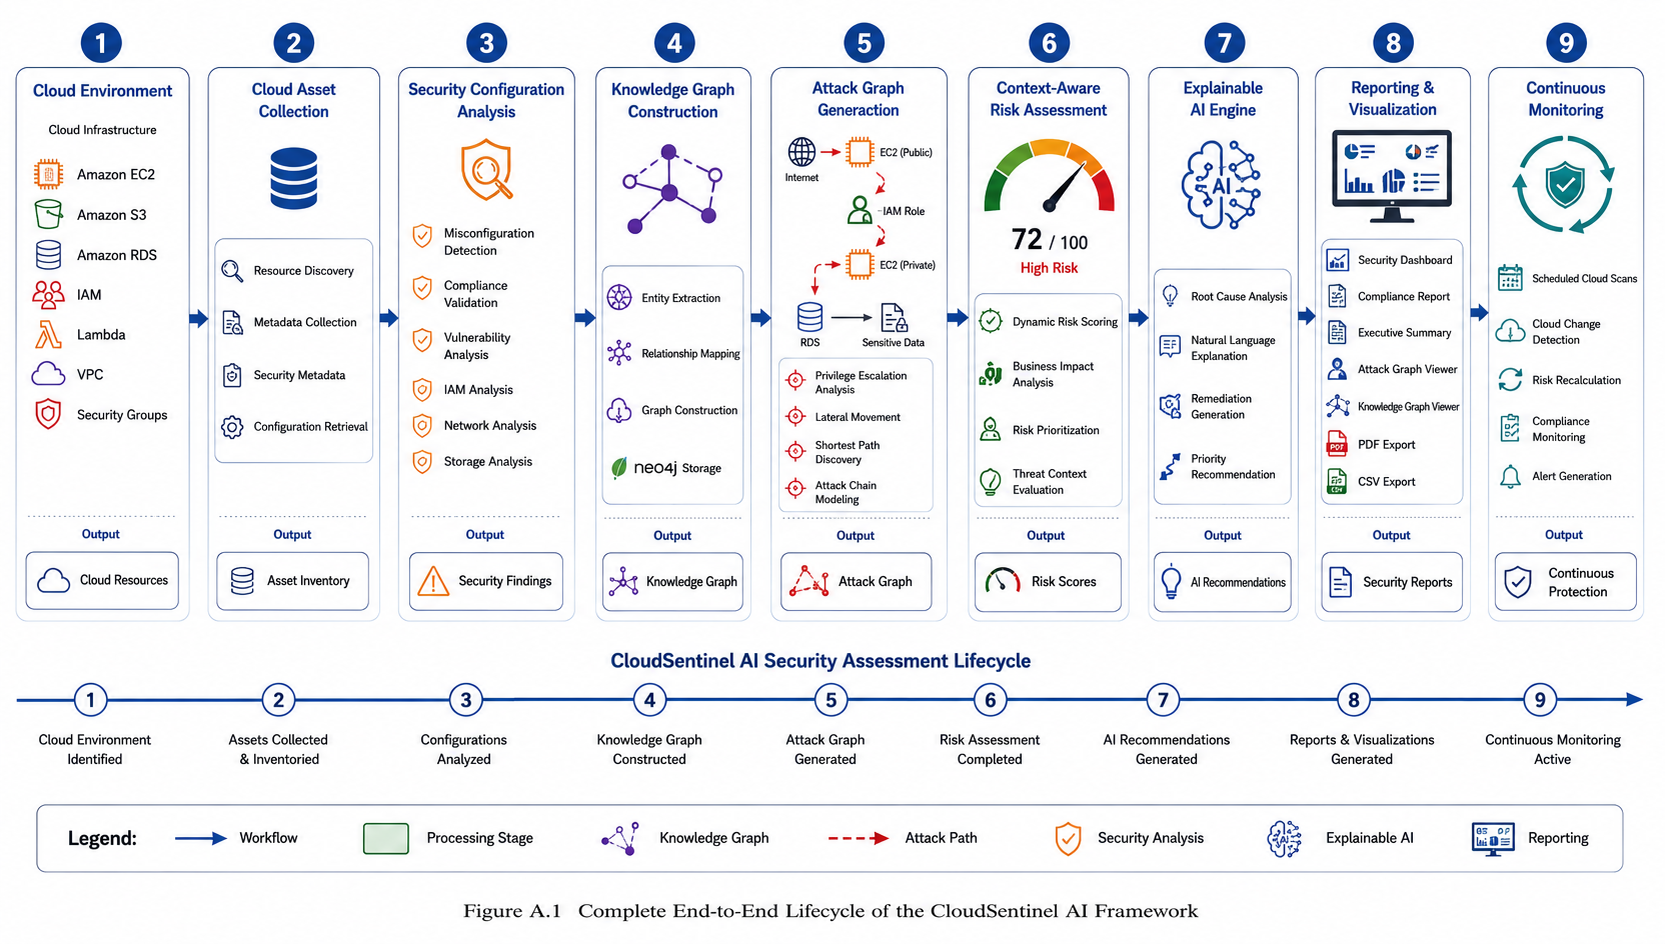
\includegraphics[width=0.9\textwidth,height=\textheight]{figures/image-a.1.png}
\caption{Appendix figure A.1.}\label{fig:a_1}
}
\end{figure}

\begin{figure}
\hypertarget{fig:a_2}{%
\centering
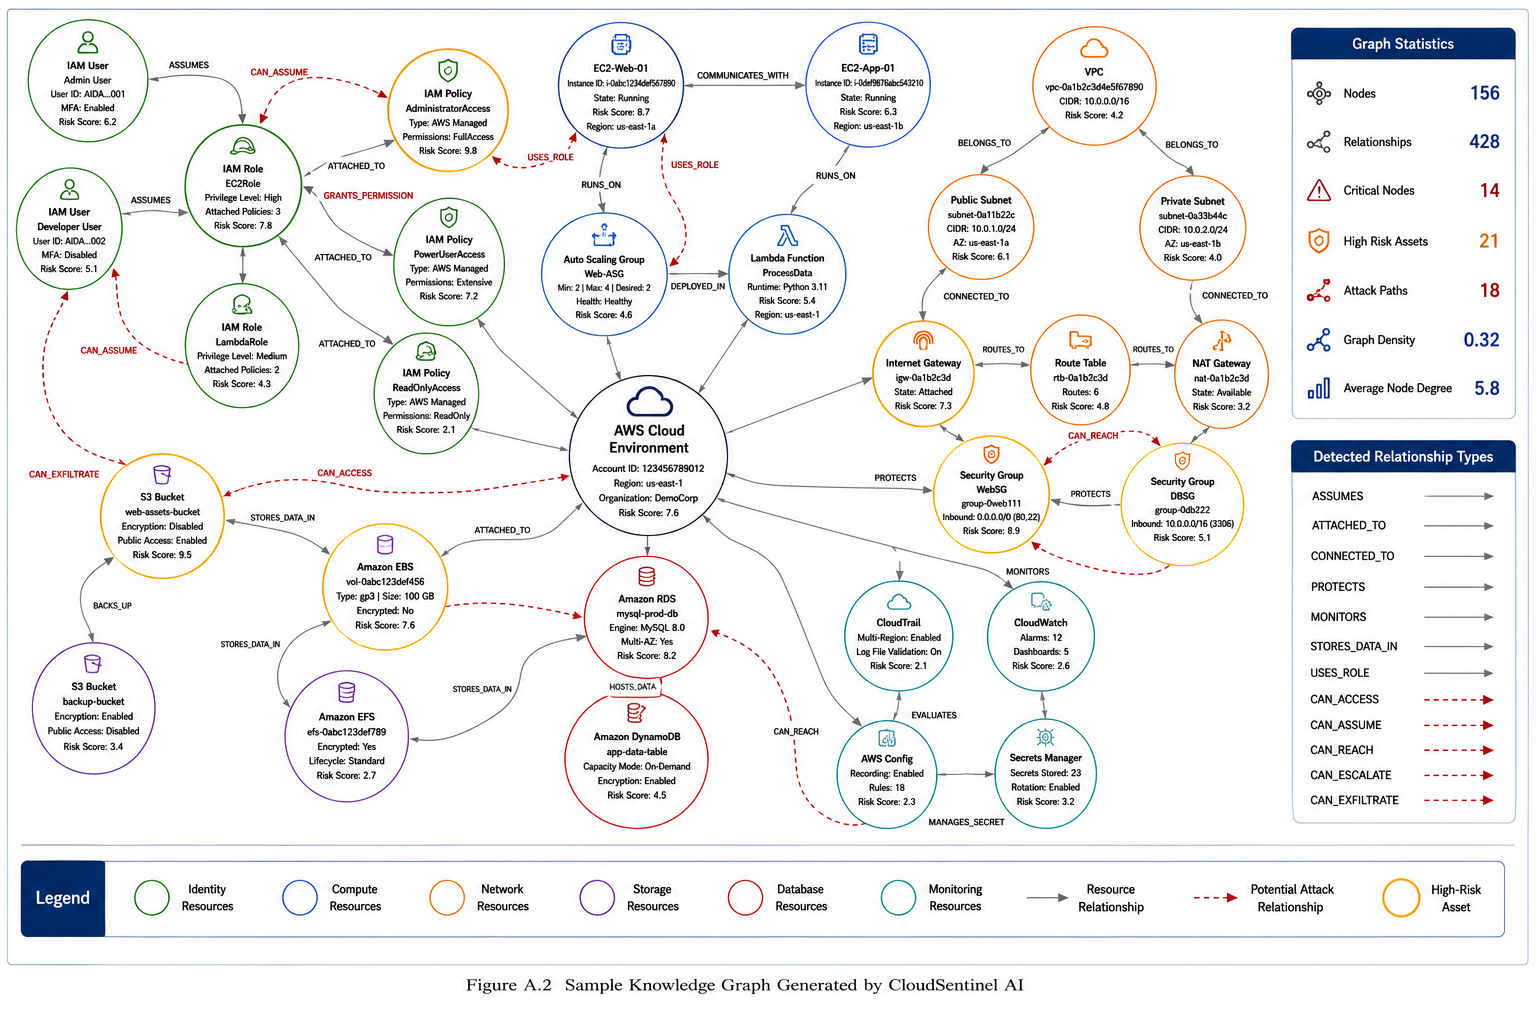
\includegraphics[width=0.9\textwidth,height=\textheight]{figures/image-a.2.png}
\caption{Appendix figure A.2.}\label{fig:a_2}
}
\end{figure}

\begin{figure}
\hypertarget{fig:a_3}{%
\centering
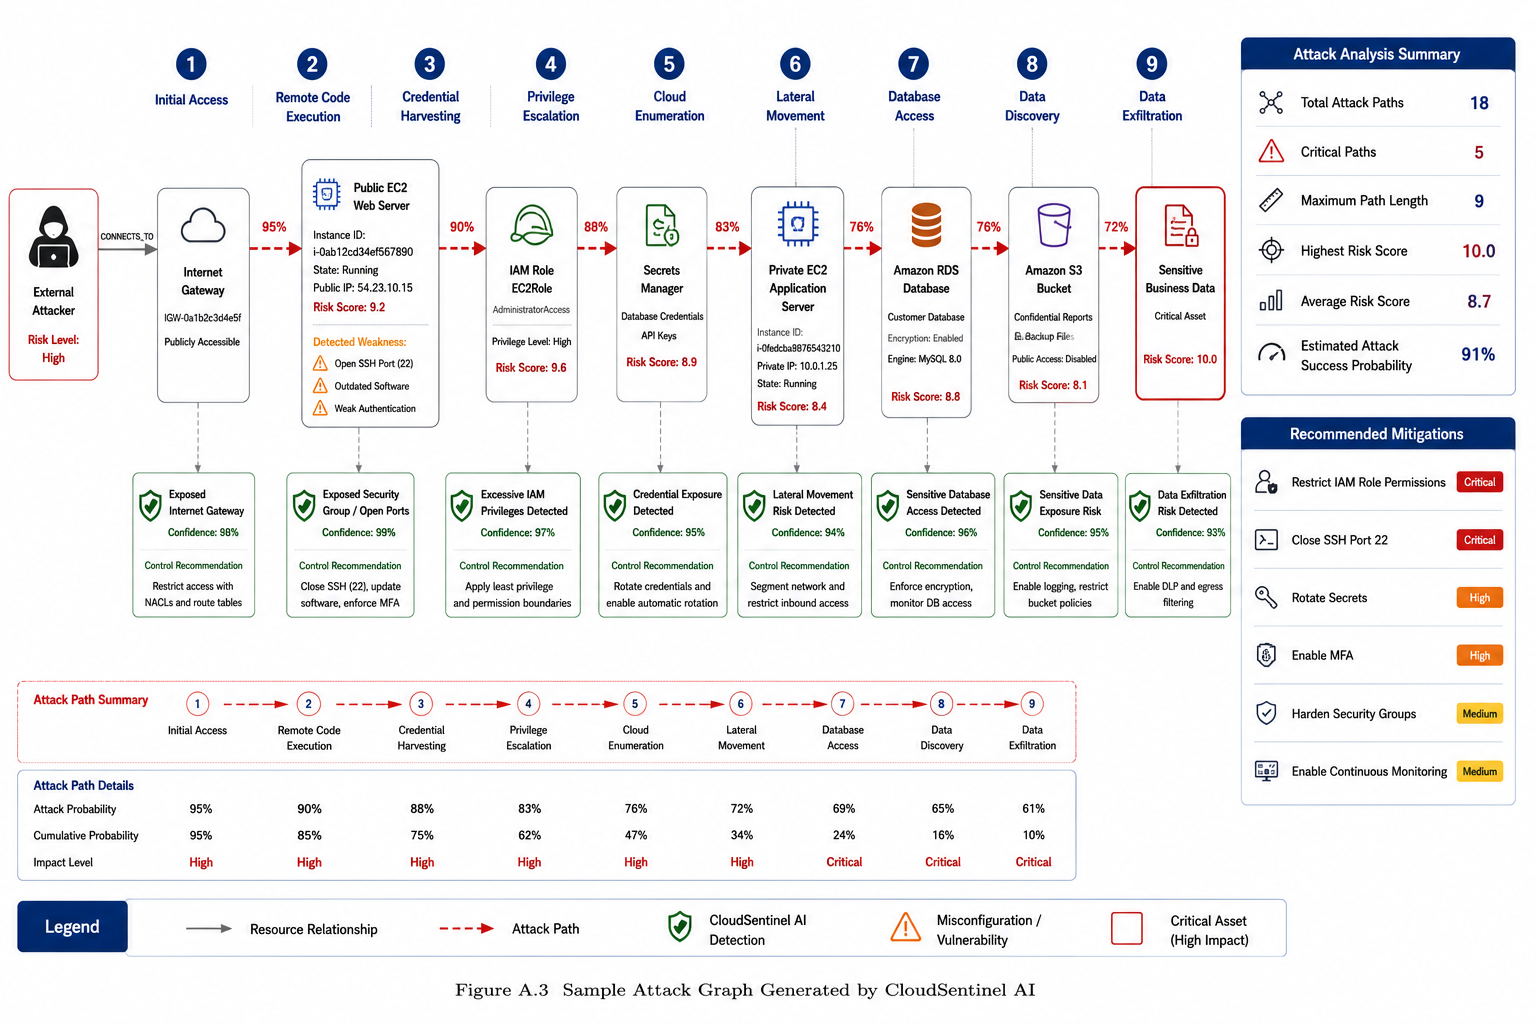
\includegraphics[width=0.9\textwidth,height=\textheight]{figures/image-a.3.png}
\caption{Appendix figure A.3.}\label{fig:a_3}
}
\end{figure}

\begin{figure}
\hypertarget{fig:a_4}{%
\centering
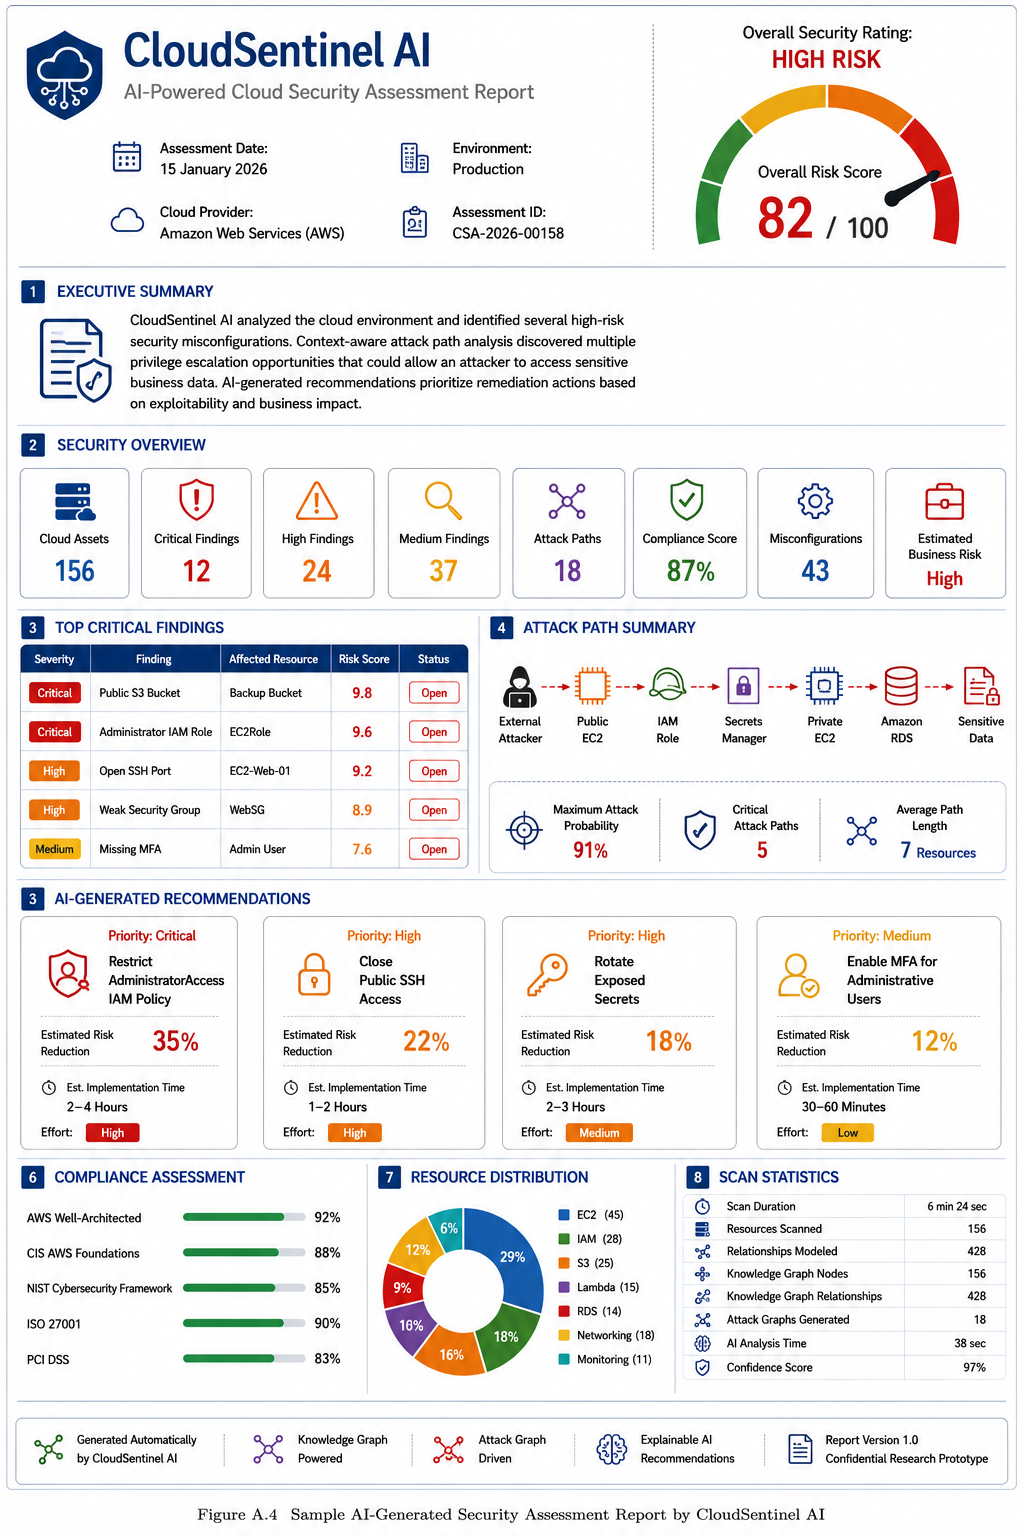
\includegraphics[width=0.9\textwidth,height=\textheight]{figures/image-a.4.png}
\caption{Appendix figure A.4.}\label{fig:a_4}
}
\end{figure}

\begin{figure}
\hypertarget{fig:a_5}{%
\centering
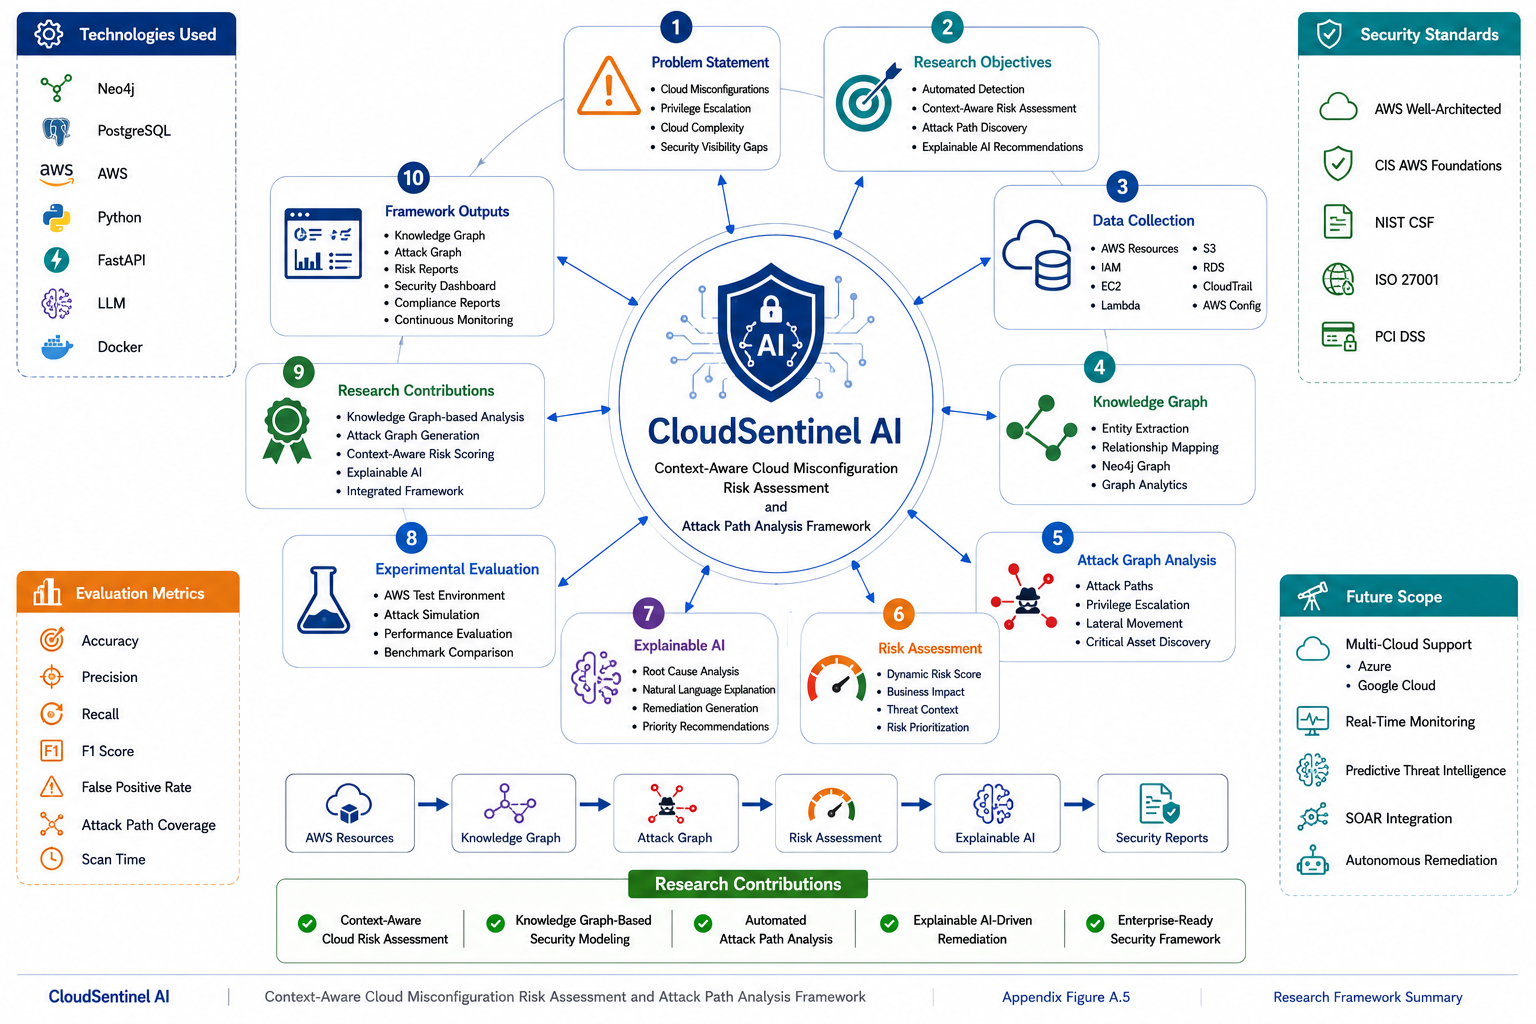
\includegraphics[width=0.9\textwidth,height=\textheight]{figures/image-a.5.png}
\caption{Appendix figure A.5.}\label{fig:a_5}
}
\end{figure}
